\documentclass[11pt,oneside,a4paper]{article}
\usepackage{graphicx}
\usepackage{booktabs}
\usepackage{caption}
\usepackage{subcaption}
\usepackage{amsmath}
\usepackage{amsfonts}
\usepackage{amssymb}
\usepackage{lscape}
\usepackage{psfrag}
\usepackage[usenames]{color}
\usepackage{bbm}
\usepackage[update]{epstopdf}
\usepackage[bookmarks,pdfstartview=FitH,a4paper,pdfborder={0 0 0}]{hyperref}
\usepackage{verbatim}
\usepackage{listings}
\usepackage{textcomp}
\usepackage{fancyhdr}
\usepackage{multirow}
\usepackage{tikz}
\usepackage{lipsum}
\usepackage{xcolor}
\usepackage{wrapfig}
\usepackage[margin=1in]{geometry}
\usepackage{pdfpages}
\newcommand{\hint}[1]{{\color{blue} \em #1}}

\makeatletter
\def\cleardoublepage{\clearpage\if@twoside \ifodd\c@page\else%
\hbox{}%
\thispagestyle{empty}%
\clearpage%
\if@twocolumn\hbox{}\clearpage\fi\fi\fi}
\makeatother

\sloppy
% \widowpenalty=10000
% \clubpenalty=10000

\title{
    \vspace*{0.0mm}
    \LARGE\bf\sf Network Security (Fall 2019)
    \vspace*{10.0mm} \\
    %
    \Huge\bf\sf Summary
    %
    \vspace*{30.0mm} \\
    \normalsize
    %
    \sf Author:\\[5pt]
    \sf Yannick Merkli\\ [5pt]
    \sf \pageref{lastpage} Pages
}
\date{}

\begin{document}

\maketitle
\thispagestyle{empty}
\raggedbottom
\clearpage

\pagenumbering{roman}

\clearpage
\setcounter{tocdepth}{2}
\tableofcontents
\clearpage
\pagenumbering{arabic}

\begin{center}
	\noindent \textbf{\LARGE Disclaimer: Legal use of the material}
	
	\noindent Some knowledge, technologies, code is usable for attacks, it is illegal to use them for criminal activities. It is also illegal to make available such technologies and code without proper measures.\\
	This summary is based on \cite{netsec}.
\end{center}


\newpage

\section{SSL, TLS, PKI}

\subsection{SSL/TLS Overview}

Goal: Secure Internet communication.\\
We need \textit{secrecy} to precent eavesdroppers from learning sensitive information and we need entity and message authentication to prevent message alteration/ injection.

\subsection{PKI overview}

In symmetric cryptography, main challenge is key distribution as keys need to be distributed via confidential and authentic channels. In public-key systems, main challenge is key authentication (i.e., which key belongs to whom) as keys need to be distributed via authentic channels.\\
\textit{Public-key infrastructures (PKIs) provide a way to validate public keys}.\\

\noindent Terminology: 

\vspace{-\topsep}
\begin{itemize}
	\setlength{\itemsep}{0pt}
	\setlength{\parskip}{0pt}
	\item PKI: Public-key infrastructures
	\item CA: Certification authority
	\item A public-key certificate (or simply certificate) is signed and binds a name to a public key \item Trust anchor, trust root: self-signed certificates of public keys that are allowed to sign other certificates.
	\item X.509: standard format of digital certificate, defines a structure for public key certificates: Two sections: data and signature section.
\end{itemize}
\vspace{-\topsep}

\noindent Trust establishment: You cannot establish trust out of thin air - we need a root of trust to establish trust in other entities. Cryptographic operations enable transfer of trust from one entity to another.

\subsection{X.509}

X.509 defines a structure for public key certificates

\vspace{-\topsep}
\begin{itemize}
	\setlength{\itemsep}{0pt}
	\setlength{\parskip}{0pt}
	\item Two sections: data and signature sec1on
	\item A CA assigns a unique name to each user and issues a signed certificate
	\item Often name is the domain or Email address
	\item Each CA issues a certificate for those beneath it
\end{itemize}
\vspace{-\topsep}

\noindent Multi-Domain Certificates are possible and used e.g. by CDNs. Content Delivery Networks (CDN) are hosting web sites for domains and thus need a certificate to service content. CDNs are obtaining a single certificate for multiple domains.

\subsection{Compelled Certificates}

Compelled certificate: public/private key pair for law enforcement (MitM attacks on TLS) with CA certificate enabling private key to sign additional certificates. Compelled certificates carry inherent risks: Since the certificates are non-repudiable, anyone who gets hold of the second valid certificate the CA's or the government's involvement in a compelled certificate creation attack. This results in a loss of trust in the CA or the government. If the CA creates an intermediary CA certificate for the government, then that certificate would have to be registered in a CT log, but in that case, the attack
does not become directly attributable to VeriSign, as the forged certificate is signed by the intermediary certificate.

\newpage

\subsection{Approaches to improve TLS}

\subsubsection{The “Let’s Encrypt” CA}

Goal: provide free certificates with automatic domain validation, issuance, and renewal. It uses relatively short-lived certificates (90 days). It is based on ACME (Automated Certificate Management Environment).

\subsubsection{Levels of trust}

Have different levels of trust in certificates:

\vspace{-\topsep}
\begin{itemize}
	\setlength{\itemsep}{0pt}
	\setlength{\parskip}{0pt}
	\item No SSL/TLS
	\item Domain validation (DV): the domain is validated but the owner could be malicious (e.g. bad.com with certificate for bad.com)
	\item Organization validation (OV) / "High assurance": A certificate provider will issue an OV class certificate to a purchaser if the purchaser can meet two criteria: the right to administratively manage the domain name in question, and perhaps, the organization's actual existence as a legal entity. (e.g. wikipedia.org)
	\item Extended validation (EV): can be issued only by a subset of certificate authorities (CAs) and require verification of the requesting entity's legal identity before certificate issuance (e.g. credit-suisse.com). They are further displayed differently in most browsers. 
\end{itemize}
\vspace{-\topsep}

\subsubsection{HTTP Strict Transport Security (HSTS)}

Goal: allows servers to declare that their clients should only use HTTPS (for a specified period). This prevents some “downgrade”, “SSL stripping”, and “session hijacking” attacks. Browsers should automatically redirect to HTTPs or display a warning message. HSTS is implemented with an HTTPS header. Example: \\
\indent \texttt{Strict-Transport-Security: max-age=31536000}\\
\noindent HSTS doesn't help at all if valid bogus certificates are used.

\subsubsection{HTTP Public-Key Pinning (HPKP)}

A server implementing HPKP will provide the client with a list of hashes of valid
certificates for the domain. This list is delivered in an HTTP header that also contains a
max-age value. The client will then “pin” those hashes — subsequent connection within the
max-age period will only succeed if the certificate offered by the server matches the pinned
hashes for that domain. A MitM with a different certificate would therefore fail. Example:\\
\indent \texttt{Public-Key-Pins: max-age=2592000; pin-sha256="..."; pin-sha256="...";\\
	\indent report-uri="...";\\
}
MiTM attacks can still succeed even with HPKP: HPKP is TOFU (Trust On First Use). If the first policy received comes from an
attacker, the browser will be happy to communicate with the bogus website and will block
the legitimate server. Also if a weak hash function is used, the attacker could generate a
certificate with a colliding hash — but in that case HPKP would be the last of our problems.\\

\noindent Further problem with HPKP: certificates can change often (e.g with Let's encrypt). If a certificate changes but users still hold the old policy (since the max-age hasn't expired yet), clients won't accept the new certificate although it is legitimate.

\newpage

\subsubsection{Certificate revocation}

Certificate revocation is a mechanism to invalidate certificates (e.g. after a private key is disclosed or after a trusted employee leaves a company). CA periodically publishes certificate revocation List (CRL).\\
Problem: CAP theorem (Consistency, Availability, tolerance to Par11on):
impossible to achieve all 3, need to sacrifice one!

\subsubsection{Online Certificate Status Protocol (OCSP)}

Online Certificate Status Protocol (OCSP) to verify certificate status, ensure certificate is valid and has not been revoked. Browsers will send certs to OCSP server for verification.\\
Problem: 
\vspace{-\topsep}
\begin{itemize}
	\setlength{\itemsep}{0pt}
	\setlength{\parskip}{0pt}
	\item “Optimistic” treatment of OCSP failure information: If OCSP server does not respond, a certificate would be considered invalid, although the certificate most likely isn't. This leads to false positives, which is annoying for browser users, that's why most browsers don't treat a non-responding OCSP server as invalid certificate.
	\item OCSP servers can be slow, which is another reason for browsers to deactivate it by default, since users otherwise may switch browsers.
	\item OCSP can leak browsing information outside of private browsing mode as Microsoft’s CryptoAPI and Apple’s Security Framework API cache OCSP responses in OS.
\end{itemize}
\vspace{-\topsep} 

\noindent Possible solution: OCSP stapling allows the presenter of a certificate to bear the resource cost involved in providing OCSP responses by appending ("stapling") a time-stamped OCSP response signed by the CA to the initial TLS handshake, eliminating the need for clients to contact the CA, with the aim of improving both security and performance.

\subsubsection{DNS-Based Authentica1on of Named Entities (DANE)}

Goal: authenticate TLS servers without a certificate authority (CA). DANE uses DNSSEC to bind certificates to names. Problem: this is heavily reliant on DNSSEC.

\subsubsection{Attack-resilient PKI (ARPKI)}

Goal: reduce trust in any single component (e.g. CA, log server, etc.). Reduce attack surface, no single point of failure.\\
ARPKI has a set of entities that audit each other's operation and disseminate misbehavior if detected:

\vspace{-\topsep}
\begin{itemize}
	\setlength{\itemsep}{0pt}
	\setlength{\parskip}{0pt}
	\item Client (browser) establishes TLS connections with	Domain
	\item Integrity Log Server (ILS) logs domains’ certificates, makes logs publicly available and maintains Integrity Tree
	\item Certification Authority (CA) certifies domains’ public keys, download ILS data and check consistency and check behavior of other CAs.
\end{itemize}
\vspace{-\topsep}

\noindent ARPKI communication flows:

\vspace{-\topsep}
\begin{itemize}
	\setlength{\itemsep}{0pt}
	\setlength{\parskip}{0pt}
	\item Domains obtain certificate with multiple signatures from different CAs
	\item CAs also act as validators to survey operation by ILSes. They download accepted requests and validate log
	\item $n$ parties are needed for valid certificate (ILS and $n-1$ parties are different CAs)
\end{itemize}
\vspace{-\topsep}

\begin{figure}[t!]
	\centering
	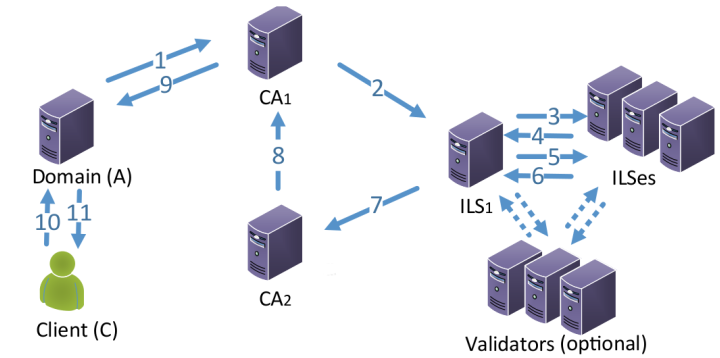
\includegraphics[width=0.5\linewidth]{figures/arpki}
	\caption{ARPKI}
	\label{fig:arpki}
\end{figure}

\newpage

\subsubsection{Certificate transparency (CT)}

Certificate	Transparency will make all public end-entity TLS certificates public knowledge,	and	will hold CAs publicly accountable for all certificates they issue. And it will do so without introducing another trusted third party.\\
\noindent CT uses a CT log that is an append-only list of certificates. The log server verifies the certificate chain (CA attribution for certificate miss-issuance and spam control). Periodically, all new certificates are appended to the append-only log and that list is then signed. All updates of the signed list of certificates ("the log") are published to the world. The CT log is implemented as a merkle hash tree. We have three participants in the protocol:

\begin{figure}
	\centering
	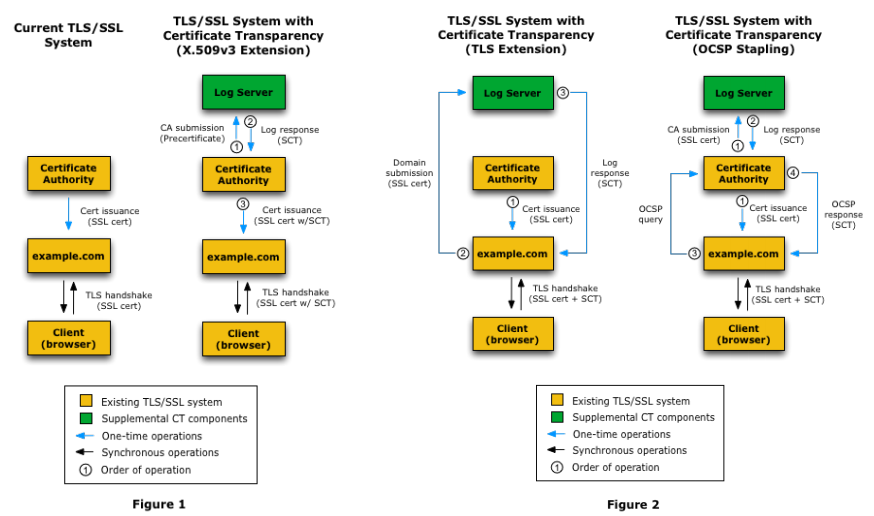
\includegraphics[width=0.9\linewidth]{figures/tls_with_ct}
	\caption{TLS with certificate transparency}
	\label{fig:tlswithct}
\end{figure}


\vspace{-\topsep}
\begin{itemize}
	\setlength{\itemsep}{0pt}
	\setlength{\parskip}{0pt}
	\item Log Server. Contains a list of certificates that is publicly available. Must
	add the certificates submitted by the CAs.
	\item Clients (auditors). Can verify the existence of certificates by checking the log server,
	and exchange information with the monitors about the log server status, in order to
	ensure the log server is not compromised.
	\item CAs (monitors). Request the addition of every newly issued cert, check that the log
	server actually adds the certificates, monitor what the other CAs are doing.
	\item Certificate owners: Query monitors to verify that nobody has logged illegitimate certs for their domain.
\end{itemize}
\vspace{-\topsep}

\newpage

\noindent Upon receiving a new certificate chain from domain or CA: the log verifies the certificate, issues a signed certificate timestamp (SCT) and promises to add the new certificate to the MHT (SCT is necessary since certs are only periodically added to log).\\
How does CT handle revocation? The certificates stay on the log forever: Merkle trees allow for easy insertion but not for immediate deletion. The current system implements revocation transparency, which is very similar to CT, but for revocation requests.\\

\noindent Disadvantages of CT:

\vspace{-\topsep}
\begin{itemize}
	\setlength{\itemsep}{0pt}
	\setlength{\parskip}{0pt}
	\item MitM attack still proceeds (but can be detected externally)
	\item Browser still needs to contact Log eventually to verify that certificate is listed in log
	\item Malicious Log server can add bogus certificate
\end{itemize}
\vspace{-\topsep}

\begin{figure}[hb]
	\centering
	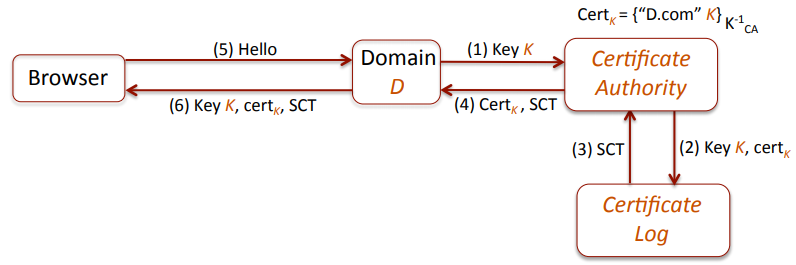
\includegraphics[width=0.6\linewidth]{figures/ct_summary}
	\caption{CT summary}
	\label{fig:ctsummary}
\end{figure}

\begin{figure}[hb]
	\centering
	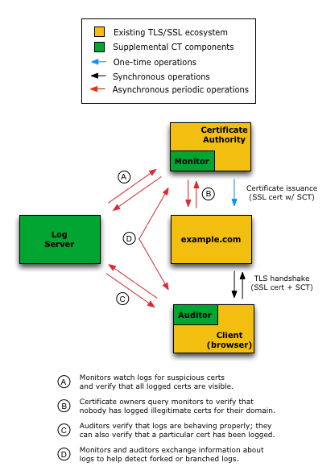
\includegraphics[width=0.5\linewidth]{figures/ct_participants}
	\caption{CT participants}
	\label{fig:ctparticipants}
\end{figure}



\newpage

\section{TLS}

Perfect forward secrecy: when obtaining a private key, I can only decrypt future sessions, not past ones.

\subsection{Cipher suites}

\texttt{TLS\_\{KEY\_EXCHANGE\}\_\{AUTHENTICATION\}\_WITH\_\{BULK\_ENCRYPTION\}\_\{MAC\}}

\noindent Example: \texttt{TLS\_DHE\_RSA\_WITH\_AES\_128\_GCM\_SHA256}\\
Key exchange: Ephemeral Diffie-Hellman, Authentication: RSA, Encryption: 128-bit AES GCM mode, MAC: 256-bit SHA-2

\subsection{Handshake protocol}

\vspace{-\topsep}
\begin{itemize}
	\setlength{\itemsep}{0pt}
	\setlength{\parskip}{0pt}
	\item Establishes keys needed by the Record Protocol, via establishment of the TLS mastersecret and subsequent key derivation.
	\item Provides authentication of server (usually) and client (rarely), using public key cryptography supported by digital certificates or pre-shared key (less common, used in IoT).
	\item Protects negotiation of all cryptographic parameters. SSL/TLS version number, encryption and hash algorithms, authentication and key establishment methods. This prevents version rollback and cipher suite downgrade attacks.
\end{itemize}
\vspace{-\topsep}

\begin{figure}[hb]
	\centering
	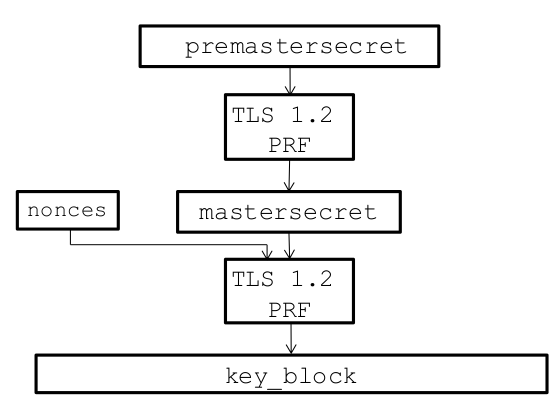
\includegraphics[width=0.4\linewidth]{figures/tls_key_derivation}
	\caption{TLS key derivation. The premastersecret is either a client-generated random-value (RSA) or the negotiated DH shared secret (DH). Nonces are public. All symmetric keys come from the key\_block (48 bytes). The split of the key\_block depends on the cipher suite.}
	\label{fig:tlskeyderivation}
\end{figure}


\subsubsection{Key establishment options}

\vspace{-\topsep}
\begin{itemize}
	\setlength{\itemsep}{0pt}
	\setlength{\parskip}{0pt}
	\item RSA: RSA key generation is expensive, that's why keys are reused. Thus, RSA does not provide perfect forward secrecy.
	\item Static Diffie-Hellman: Server certificate contains DH parameters (group, generator g)
	and static DH value $g^x$. Client chooses y, computes $g^y$ and sends to server. $$premastersecret = g^{xy}$$
	Thus, Static Diffie-Hellman does not provide perfect forward secrecy.
	\item Anonymous Diffie-Hellman: Each side sends Diffie-Hellman values in group chosen by
	server, but no authentication of these values. Vulnerable to man-in-middle attacks even if only offered.
	\item The key exchange is called “ephemeral” if the client and server both choose a new key pair for every exchange. Ephemeral key exchanges offer PFS.
	\item (EC)DHE: Offers perfect forward secrecy.
\end{itemize}
\vspace{-\topsep}

\newpage

\subsection{Record protocol}

TLS Record Protocol uses symmetric encryption, using the keys negotiated during the handshake protocol. It provides:

\vspace{-\topsep}
\begin{itemize}
	\setlength{\itemsep}{0pt}
	\setlength{\parskip}{0pt}
	\item Data origin authentication, integrity using a MAC.
	\item Confidentiality using a symmetric encryption algorithm.
	\item Anti-replay using sequence numbers protected by the MAC.
	\item Optional compression.
	\item A stream-oriented API for applications making use of it.
	\item Hence TLS may fragment into smaller records or coalesce into larger records any data supplied by the calling application.
\end{itemize}
\vspace{-\topsep}

\noindent Different record layer encryption schemes:

\vspace{-\topsep}
\begin{itemize}
	\setlength{\itemsep}{0pt}
	\setlength{\parskip}{0pt}
	\item AES is secure in both 128-bit and 256-bit mode (and more), however if CBC mode is used, padding oracle attacks are possible. GCM mode is secure.
	\item DES is not secure.
	\item RC4 is not secure (see \ref{attack_on_rc4})
\end{itemize}
\vspace{-\topsep}

\noindent The TLS record protocol uses MAC-then-encrypt: this is \textit{really really bad} since this opens up the possibility of padding oracle attacks!

\begin{figure}[hb]
	\centering
	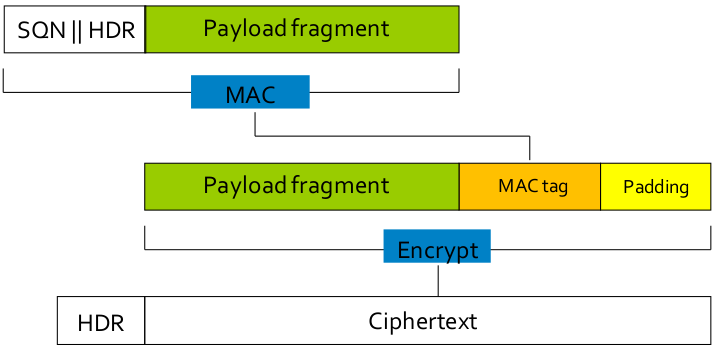
\includegraphics[width=0.4\linewidth]{figures/tls_record_protocol}
	\caption{TLS Record Protocol: MAC-Encode-Encrypt}
	\label{fig:tlsrecordprotocol}
\end{figure}

\subsubsection{TLS Record Protocol Sequence Numbers}

When the handshake is done, both client and server set the sequence number to 0 and start counting. Sequence number is 64 bits in size and is incremented for each new message. Once we reach the top (overflow), we throw away the keys and rerun the handshake (however this will rarely happen.. $2^{64}$ is very large).\\
Server and client both each maintain a copy of two seq. numbers: one for sending, one for receiving. Sequence numbers are not transmitted as part of message (TCP already provides reliable transport), however they are included in the MAC. Sequence numbers and MAC together give replay protection.\\
A wrong sequence number leads to a failure of the MAC verification. TLS is thus reliant on TCP to deliver messages in order.


\newpage

\section{Attacks against TLS}

\subsection{Attack on RC4}
\label{attack_on_rc4}

In RC4, we have biases towards certain byte values in the first 256 bytes of the RC4 cipher outputs. For example, at position 16, byte 240 is much more likely.\\
By analyzing \textbf{many} ciphertexts, we can do bayesian analysis and check which byte was most likely at each position. This then allows to recover the plaintext. For example, we could analyze the values at position 16 and XOR the most likely value with 240, which gives the plaintext.\\
An example on how to exploit this is: You want to target a secure cookie in the HTTPS session between a client running a web browser B and a web server W . You know W serves secure cookies over HTTPS, and you control a second web server, E, the client visits. The client will run javascript code served from E. While this code cannot directly access cookies from W (due to the same-origin policy, SOP), it can make requests to W : the cookies will be automatically attached by the browser to the new requests. The javascript can repeat enough requests to make the attack succeed — allowing the attacker to recover the plaintext cookie.

\subsection{FREAK attack}

\begin{figure}[hb]
	\centering
	\begin{subfigure}[t]{.5\textwidth}
		\centering
		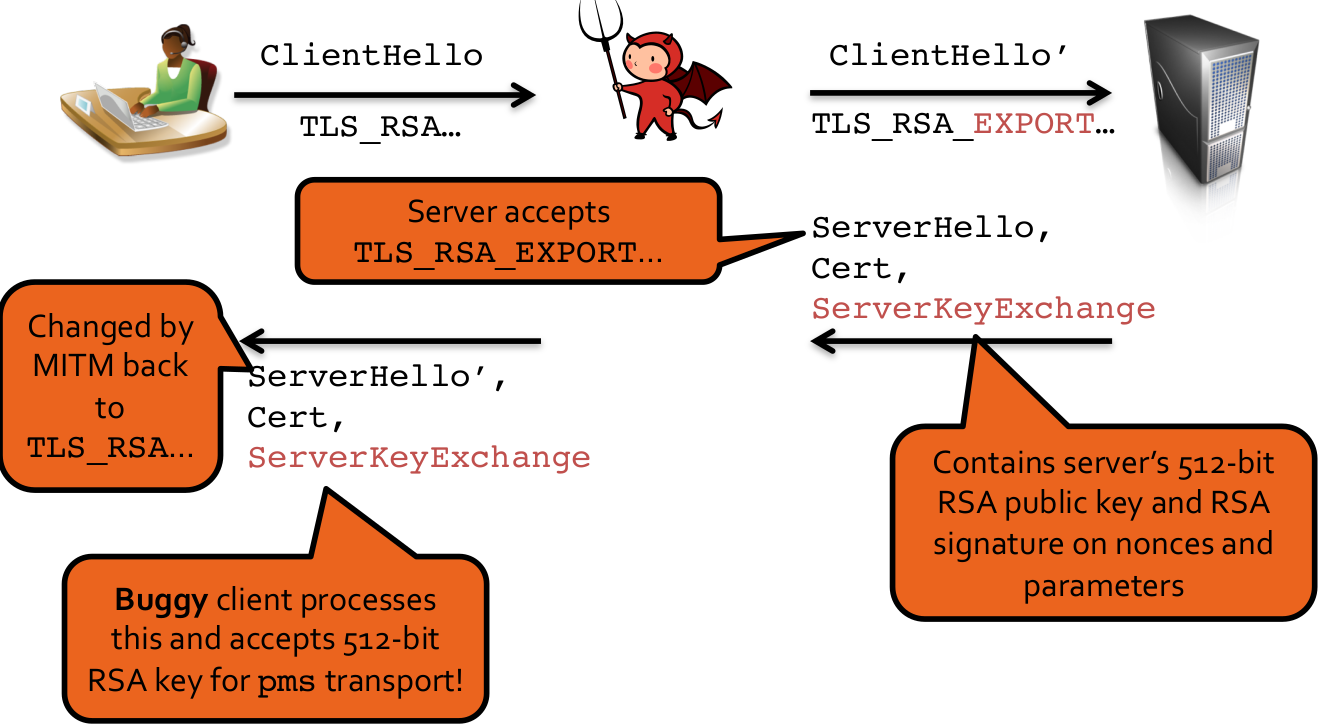
\includegraphics[width=\linewidth]{figures/tls_freak_1}
		\label{fig:tls_freak_1}
	\end{subfigure}%
	\begin{subfigure}[t]{.5\textwidth}
		\centering
		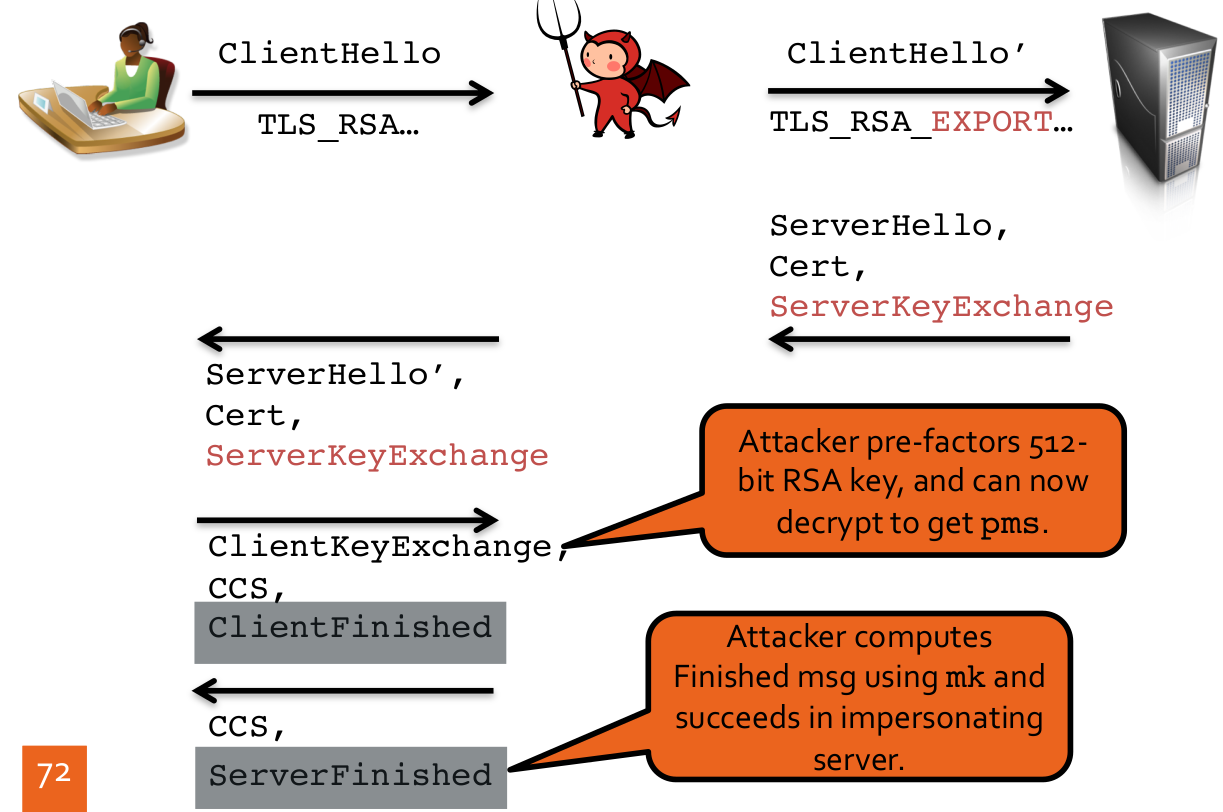
\includegraphics[width=\linewidth]{figures/tls_freak_2}
		\label{fig:tls_freak_2}
	\end{subfigure}
\end{figure}

In a FREAK attack, an active MiTM attacker forces a TLS session to use insecure export ciphers. Export ciphers are intentionally weak ciphers that were offered by the US in the 90s. During that time, these ciphers were only breakable with huge resources and a large budget. Today, they are breakable with 100\$ of AWS credit.\\
The active MiTM attacker alters the unencrypted ClientHello message to request Export RSA as the
cipher suite. Similarly, ServerHello message is changed to reflect the original ClientHello. The ServerFinished message also needs to reflect the original ClientHello and ServerHello, with the unchanged cipher suite, otherwise the client would fail transcript verification.\\
The attacker needs to be able to pre-factor the RSA key, (or factor an on-the-fly RSA key “in real time”) and craft a new ServerFinished message, removing the original from the communication channel. Since servers reuse RSA keys, the attacker can just connect to the server in advance and factor the key. Once the attacker has the key, she can decrypt the pre-mastersecret and then generate the mastersecret, using the nonces (which are in plaintext, thus public).\\
This attack was only possible due to buggy TLS client: when requesting export RSA, the server responds with a ServerKeyExchange message which contain the RSA pubKey and RSA signatures on nonces and parameters. For normal RSA (which the client thinks he's using) we would not get this message. Buggy TLS client accepted the weak key and used it, even though a different cipher was requested.\\
FREAK requires an active MiTM. The attacker needs to keep impersonating the server for all new sessions or for possible future CCS+Finish.

\subsection{Heartbleed}

The Heartbeet protocol of TLS is equivalent to ping (icmp), just for TLS. You send a msg to a server, server sends the exact msg back. Turns out, OpenSSL didn't do proper bound checking on the received msg. If you send a short msg but tell the server it's a long message, the server would send a long msg. The server would then just read over the buffer and read into memory. By doing this over and over (and being lucky) you could receive sensitive data such as passwords or private keys.

\subsection{Apple \texttt{goto fail}}

\begin{figure}[hb]
	\centering
	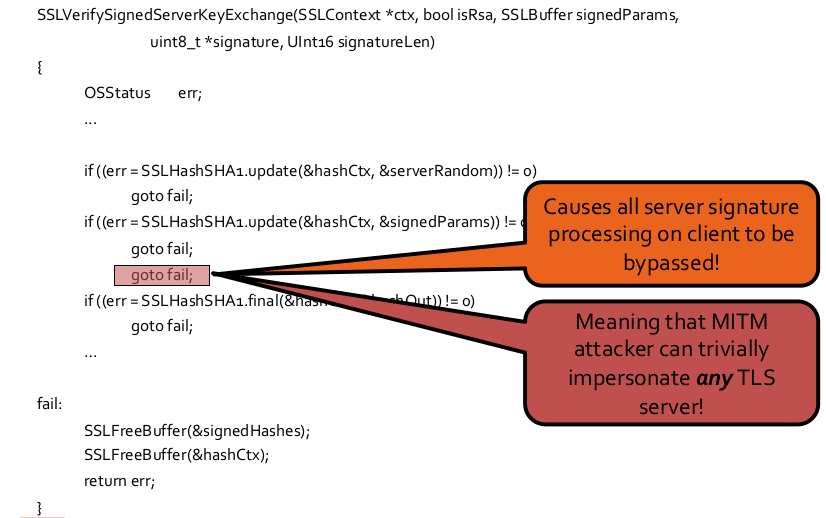
\includegraphics[width=0.5\linewidth]{figures/apple_goto_fail}
	\caption{Apple goto fail in iPhone and Mac TLS library}
	\label{fig:applegotofail}
\end{figure}

\section{TLS 1.3}

Main objectives of TLS 1.3:

\vspace{-\topsep}
\begin{itemize}
	\setlength{\itemsep}{0pt}
	\setlength{\parskip}{0pt}
	\item Protocol simplification (reducing options and removing broken cipher suites).
	\item Reduce latency of initial secure data communication (1-RTT and 0-RTT for resumed sessions).
	\item Improve security and privacy.
	\item Remove compression, RC4, MAC-then-Encrypt, RSA key transport,	custom DH and ECDH groups, renegotiation.
	\item A stream-oriented API for applications making use of it.
	\item Hence TLS may fragment into smaller records or coalesce into larger records any data supplied by the calling application.
\end{itemize}
\vspace{-\topsep}

\subsection{TLS 1.3 1-RTT handshake}

Basic idea: client sends Hello message which already includes its DH pubKey $g^x$. For this to work, the client needs to guess which DH groups the server supports.
Assuming the server actually supports the DH group it sends a ServerHello with the server DH pubKey AND it can already encrypt data since the server knows the nonces and both DH values.
DH and ECDH groups: A limited set of DH and ECDH groups are supported in TLS 1.3. This reduces likelihood of fall-back to 2-RTT and removes complexity from implementations.

\subsection{TLS 1.3 - Resumption}

Resumption uses pre-shared keys (PSK) which were established in prior session. The client sends a list of PSK IDs, one of which is selected by the server.

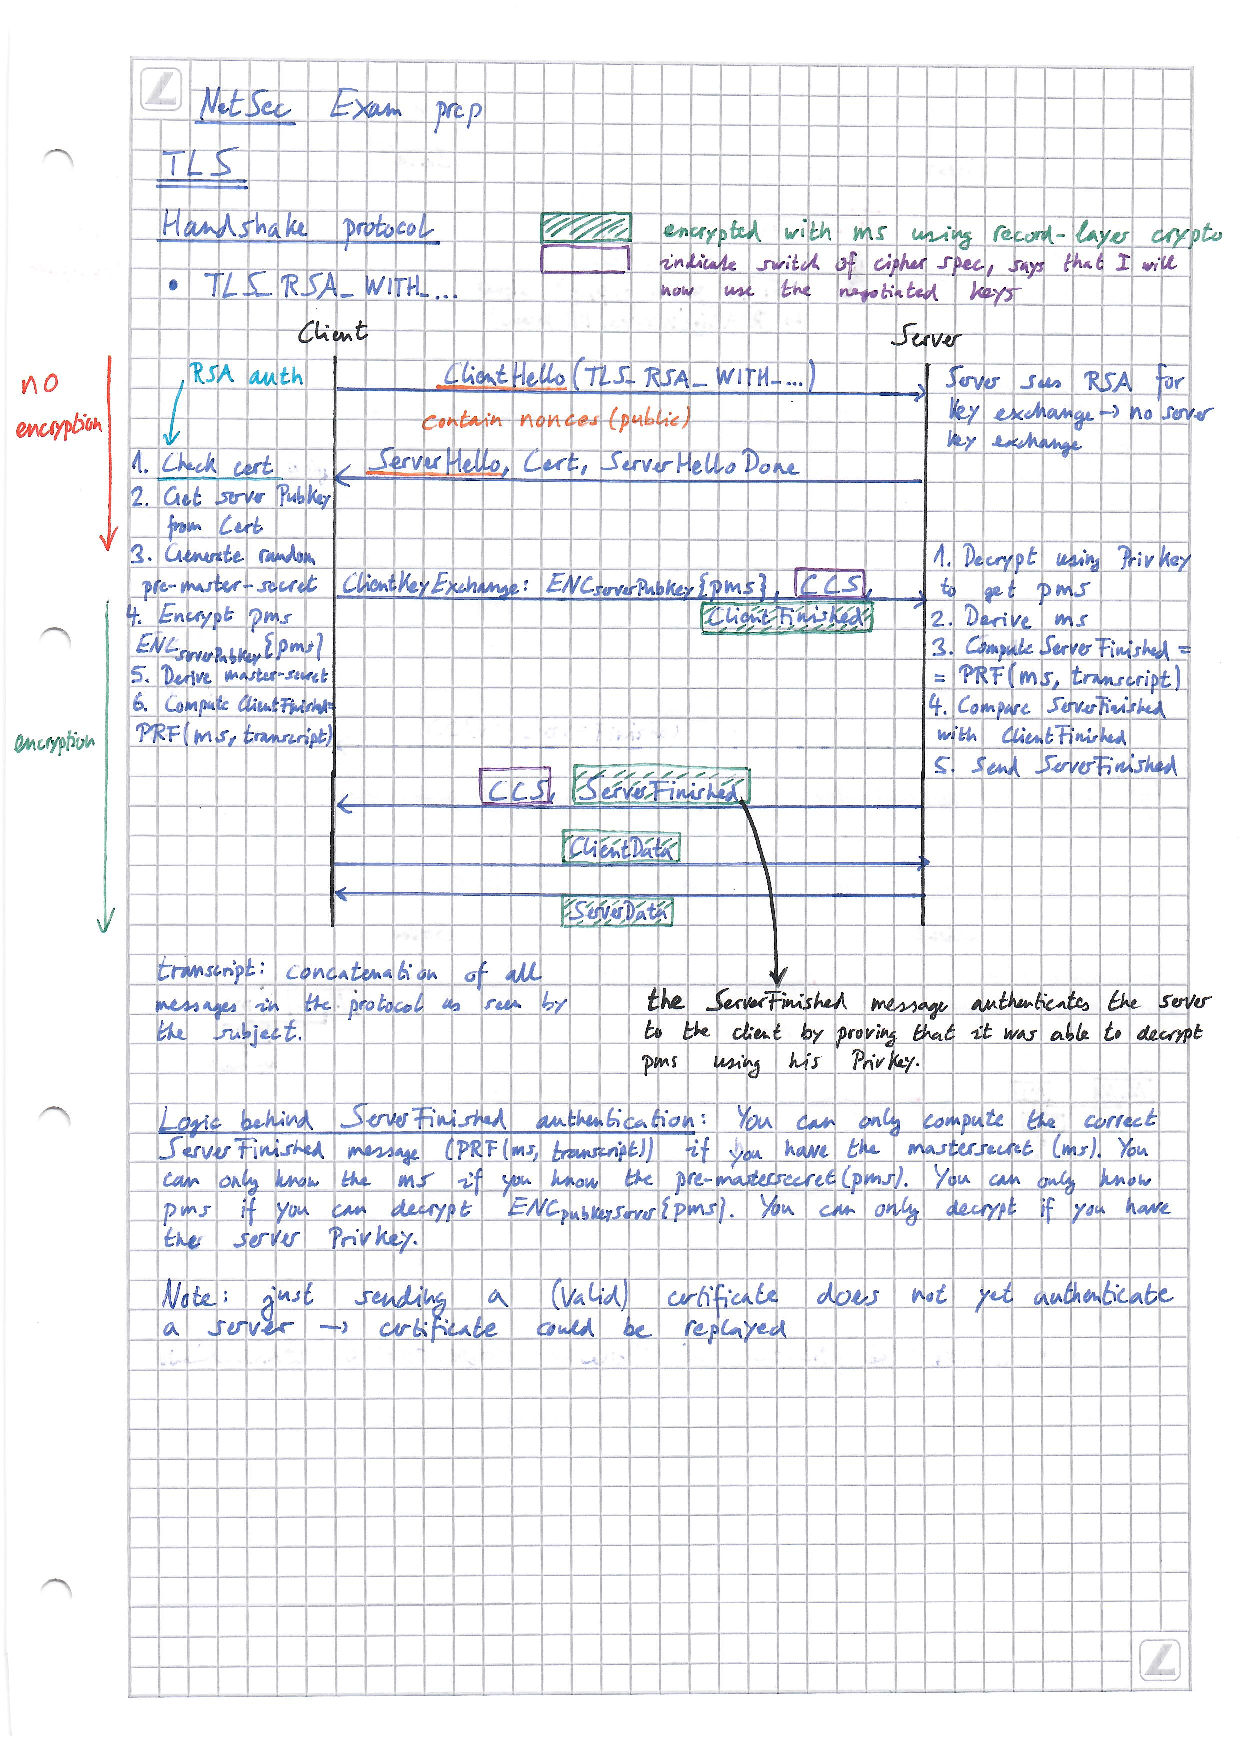
\includepdf{doc/tls_summary_1}

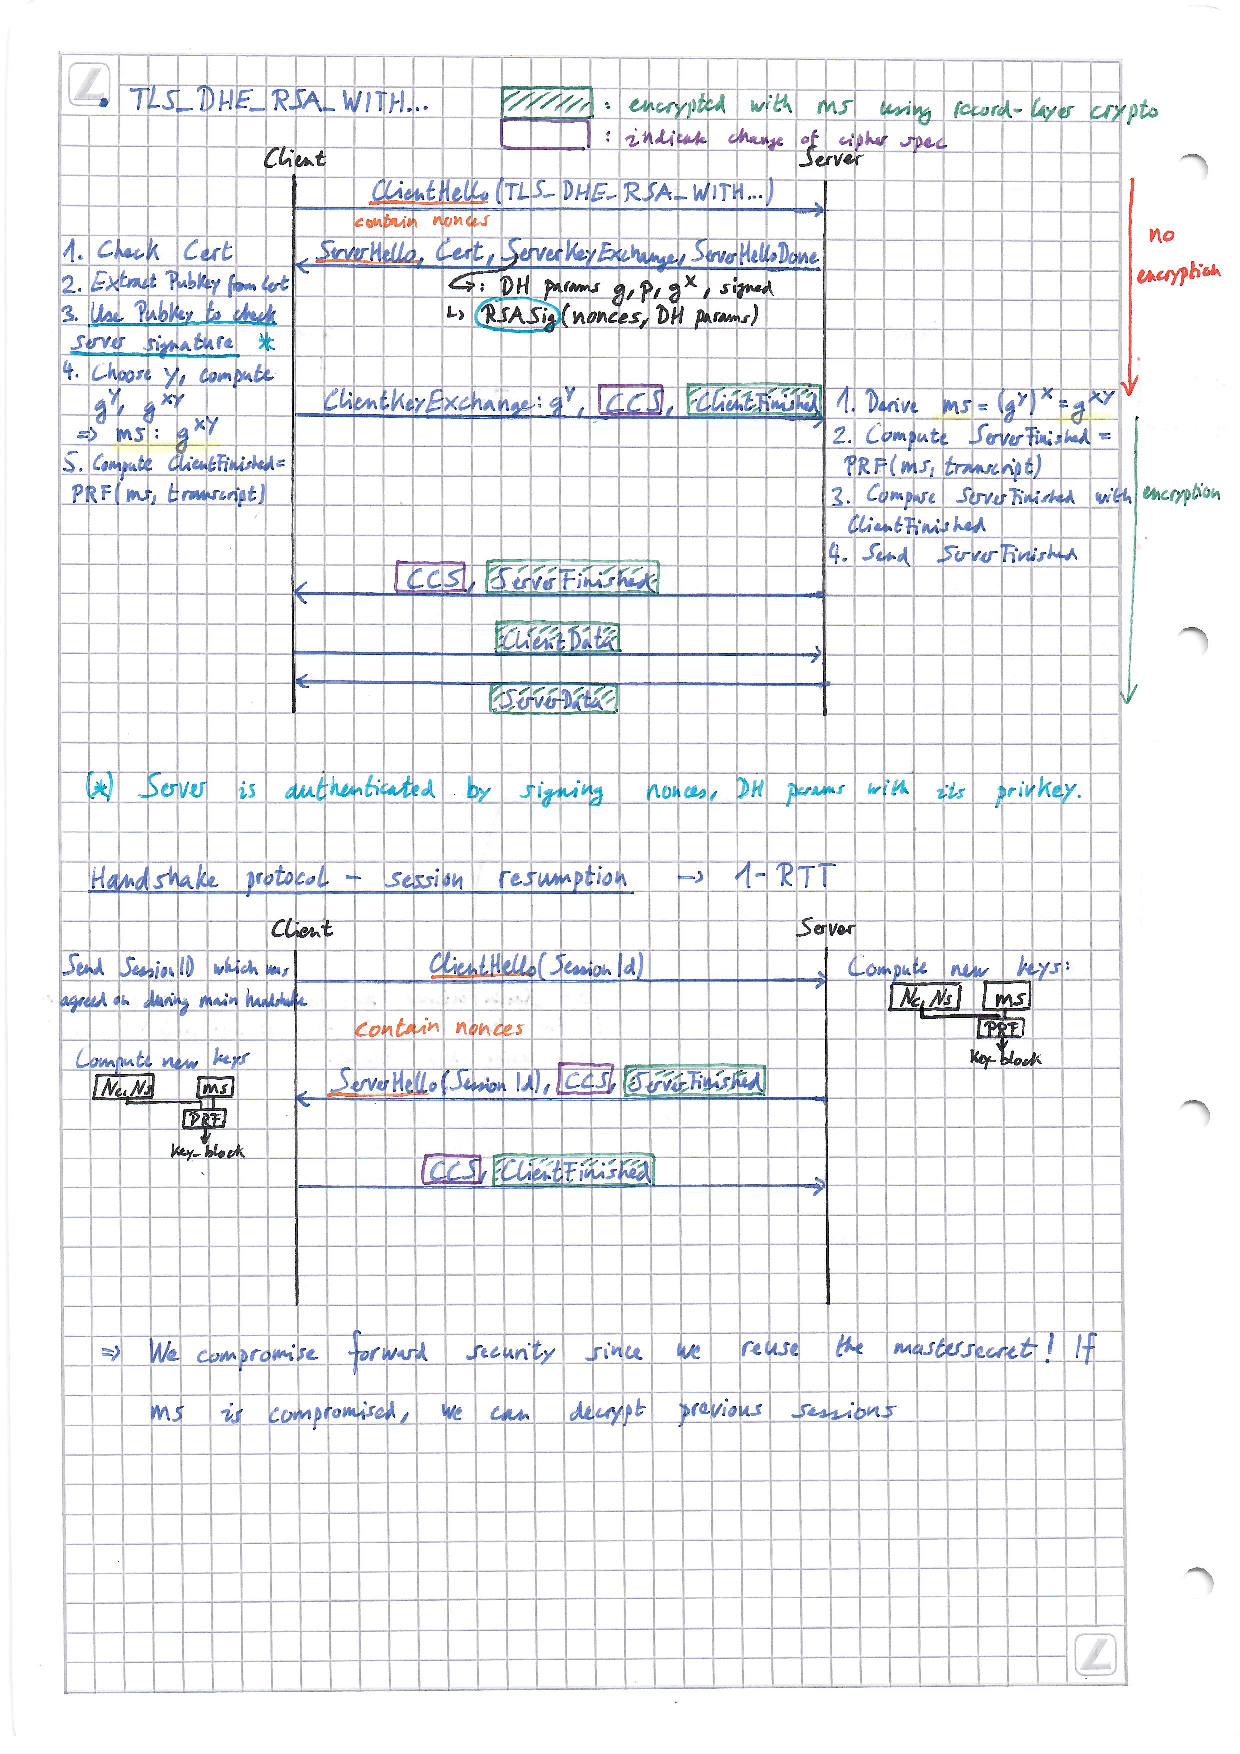
\includepdf{doc/tls_summary_2}

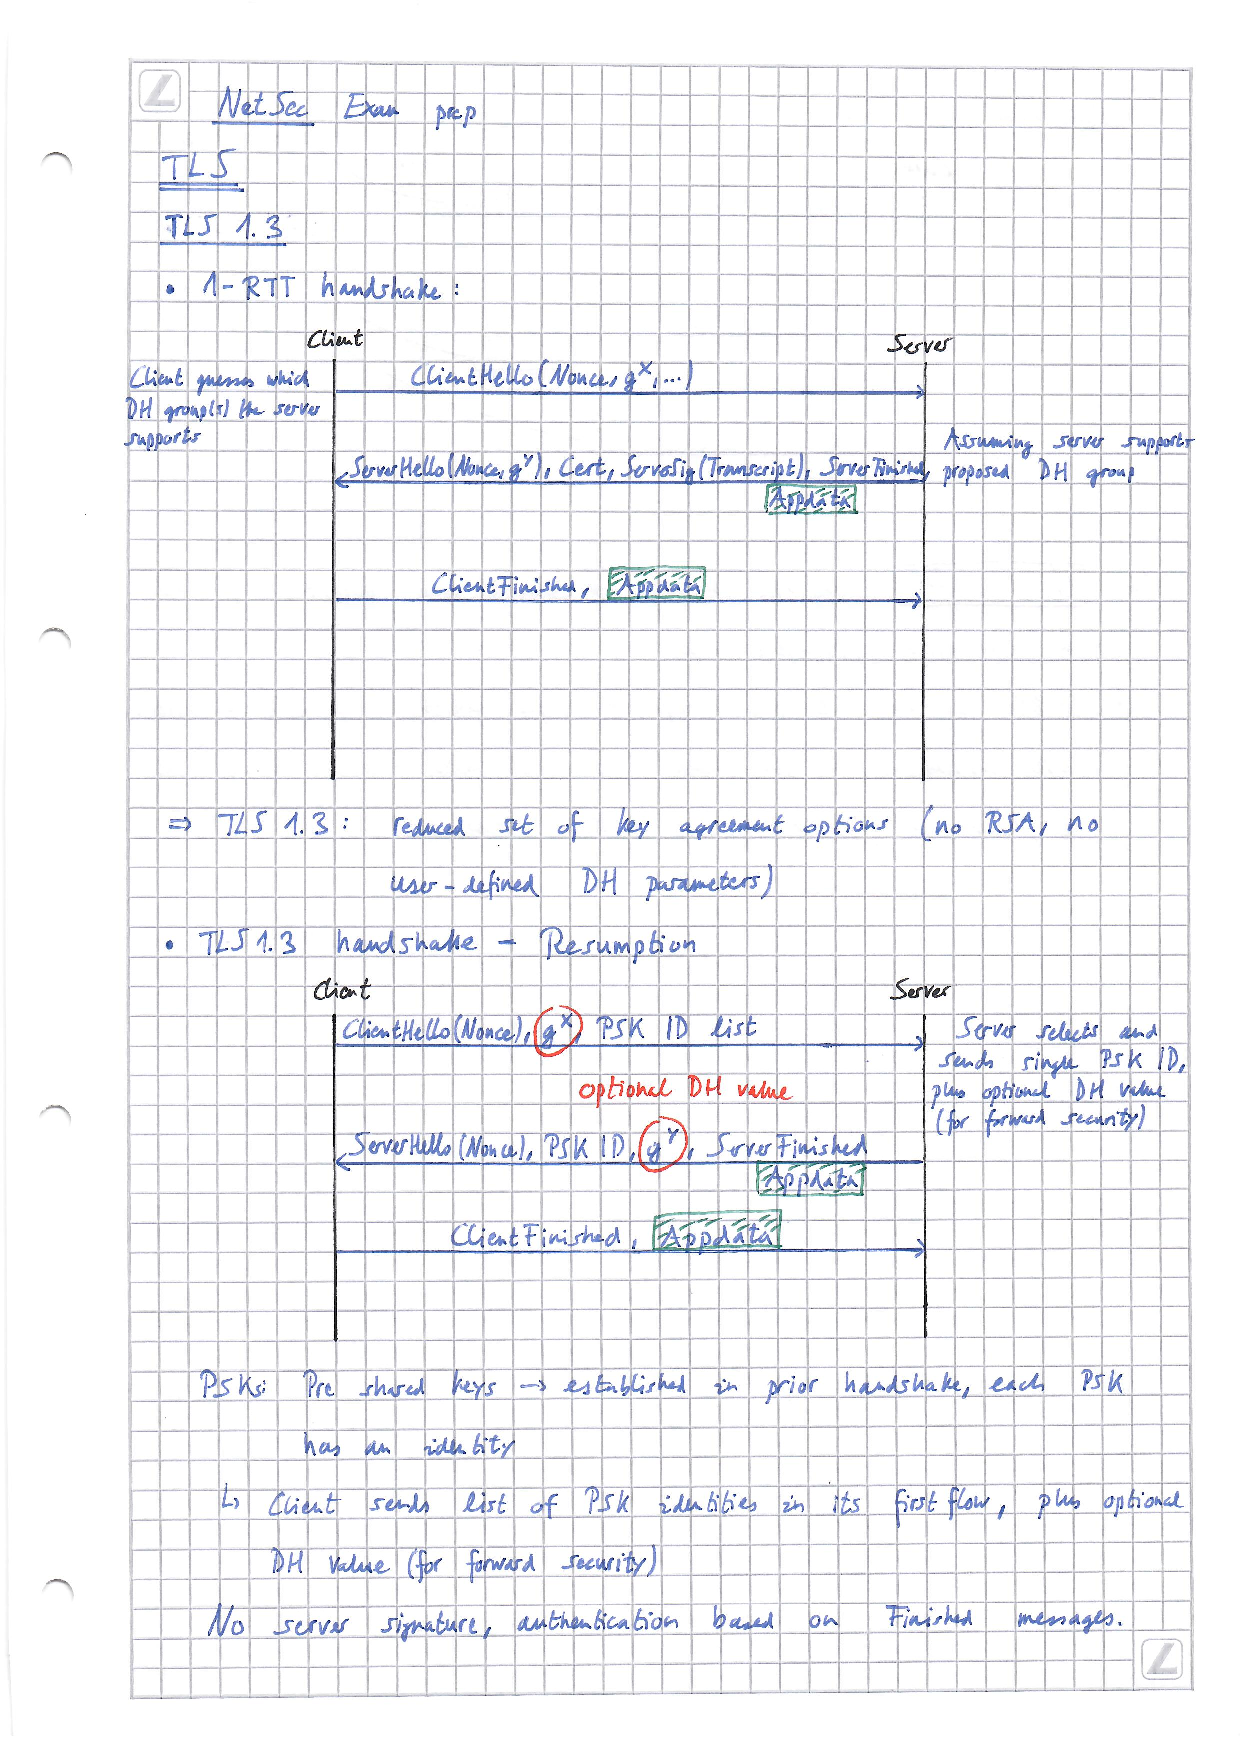
\includepdf{doc/tls_summary_3}

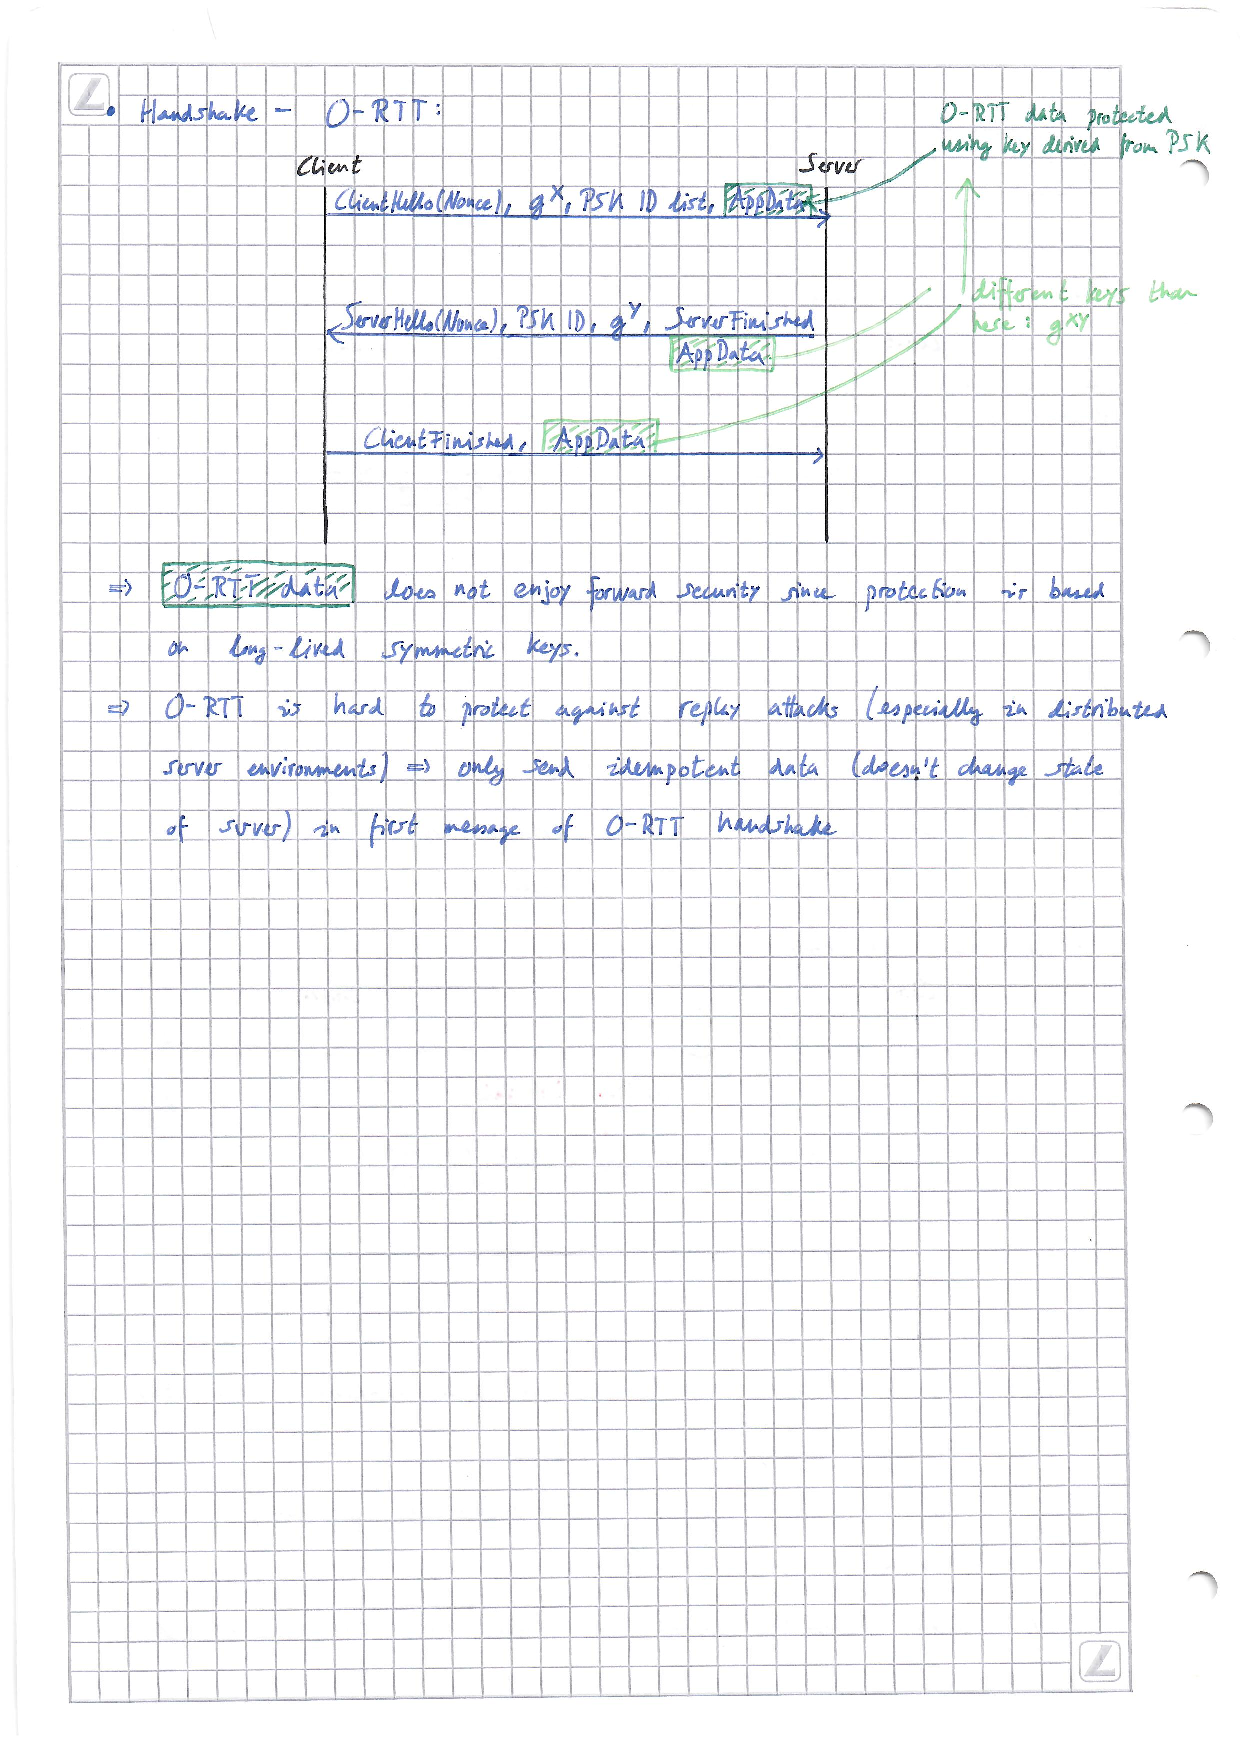
\includepdf{doc/tls_summary_4}

\section{VPNs}

A VPN creates a secure channel between two networks over an untrusted network (the Internet). VPNs and end-to-end security (TLS) complement each other. Many different VPN protocols and applications exist (IPsec, Strongswan, OpenVPN, WireGuard, ...)
Typical properties of VPN tunnels:

\vspace{-\topsep}
\begin{itemize}
	\setlength{\itemsep}{0pt}
	\setlength{\parskip}{0pt}
	\item Similar security properties as the TLS record protocol:
	\begin{itemize}
		\item Authentication of the source, integrity (MACs)
		\item Confidentiality (symmetric encryption)
		\item Replay suppression (sequence numbers)
	\end{itemize}
	\item Some tunneling protocols do not provide encryption or authentication
\end{itemize}
\vspace{-\topsep}

\noindent Typical VPN setups:

\vspace{-\topsep}
\begin{itemize}
	\setlength{\itemsep}{0pt}
	\setlength{\parskip}{0pt}
	\item secure connection between two physically separated networks (site-to-site)
	\item secure connection of a remote host to company/university network (host-to-site)
	\item VPN as a “secure” proxy (avoid tracking, spoof location, circumvent censorship)
\end{itemize}
\vspace{-\topsep}

\noindent \textbf{Why do we need VPNs when we have TLS?}

\vspace{-\topsep}
\begin{itemize}
	\setlength{\itemsep}{0pt}
	\setlength{\parskip}{0pt}
	\item If we only want to operate on layer 3 (e.g. company printer network) and still be secure
	\item When only using TLS: we still leak metadata
	\item HTTPS doesn't hide layer 3 information (srcIP, dstIP)
	\item VPNs protect all traffic ('blanket' security): DNS requests, accessing webservers without TLS
	\item VPNs can give access to services in private networks or behind firewalls
	\item VPNs allow to spoof your location
\end{itemize}
\vspace{-\topsep}

\noindent \textbf{Why do we need TLS when we have VPNs?}

\vspace{-\topsep}
\begin{itemize}
	\setlength{\itemsep}{0pt}
	\setlength{\parskip}{0pt}
	\item With VPNs, data is only secure inside the tunnel. But the data needs to somehow get to and from the tunnel. VPNs provide no security outside the tunnel
	\item VPN server can see all unencrypted traffic. TLS is still necessary.
	\item With a VPN it is not possible to authenticate a webserver, only the tunnel endpoint.
	\item VPNs need initial credential setup, TLS can be setup without knowing each other
\end{itemize}
\vspace{-\topsep}

\noindent There are many different VPN protocols but only one TLS. Why?
Because TLS is universal, everybody should be able to access webservers securely through TLS.  We thus need a globally universal standard. VPNs are setup by companies, universities, private person etc. and it only affects their clients, employees etc.. For VPNs, we can thus use whatever we want.

\subsection{IPsec}

IPsec is a very large and complicated protocol. The tunnel is setup at layer 3 (network). In IPsec, we also use sequence numbers (like in TLS) \textit{but} they are included in the packets (while TLS doesn't include sequence numbers in the packet). That's because IPsec runs on top of IP and IP is best-effort transport. The ordering of packets can thus be off at the receiver. That's why sequence numbers need to be in the packets. What if we are tunneling UDP traffic?
The numbers are also there to avoid replay attacks. Each party has a sliding window so that it can
detect if a packet is replayed by inspecting the sequence number.

\subsubsection{Internet key exchange (IKEv2)}

IKE is used to setup a security association (SA). In IKE, we have an anonymous DH exchange. This provides forward security and does not leak identities (as e.g. TLS does) since no authentication data is sent in plaintext. The disadvantage is that anonymous DH is vulnerable to an active MiTM attack.

\begin{figure}[t!]
	\centering
	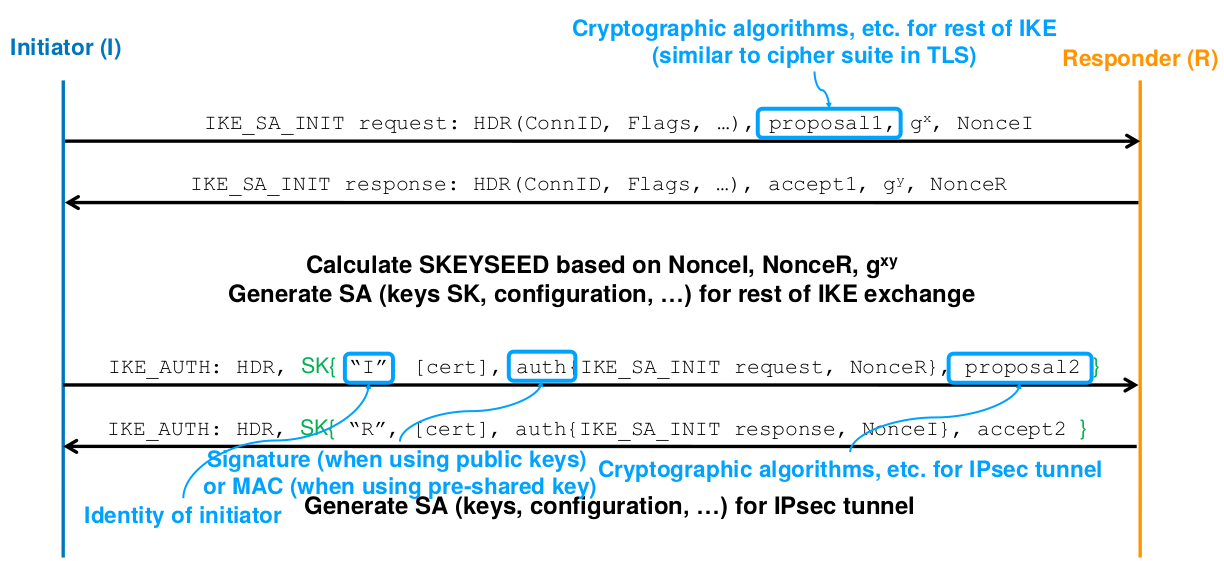
\includegraphics[width=0.9\linewidth]{figures/ikev2}
	\caption{Internet key exchange (IKEv2)}
	\label{fig:ikev2}
\end{figure}

\subsubsection{IPsec session}

After an SA was setup using IKE, we encapsulate packets and tunnel them between SA endpoints. Encapsulation works as follows:

\vspace{-\topsep}
\begin{itemize}
	\setlength{\itemsep}{0pt}
	\setlength{\parskip}{0pt}
	\item Add ESP trailer: Padding, type encapsulated (original) packet
	\item Encrypt packet and trailer
	\item Add ESP header: SA identification, sequence number
	\item Create Integrity Check Value (ICV): MAC over original packet, ESP	header, ESP trailer
	\item Add new IP header
\end{itemize}
\vspace{-\topsep}

\begin{figure}
	\centering
	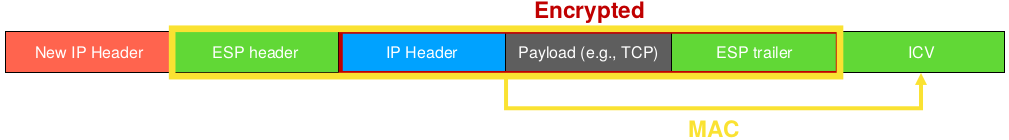
\includegraphics[width=0.7\linewidth]{figures/ipsec_encapsulation}
	\caption{IPsec encapsulation security payload (ESP) in tunneling mode}
	\label{fig:ipsecencapsulation}
\end{figure}

\noindent Similarly, decapsulation:

\vspace{-\topsep}
\begin{itemize}
	\setlength{\itemsep}{0pt}
	\setlength{\parskip}{0pt}
	\item Strip off outer IP header
	\item Look up keys and configuration using information in ESP header
	\item Check MAC
	\item Strip off authentication tag and ESP header
	\item Decrypt original packet
	\item Remove ESP trailer
	\item Forward original packet
\end{itemize}
\vspace{-\topsep}

\begin{figure}[hb]
	\centering
	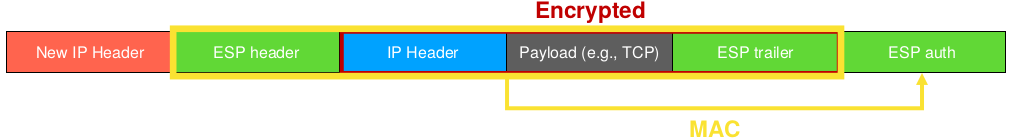
\includegraphics[width=0.7\linewidth]{figures/ipsec_decapsulation}
	\caption{IPsec decapsulation and decryption}
	\label{fig:ipsecdecapsulation}
\end{figure}

\subsection{Wireguard}

WireGuard is a modern lightweight VPN that only has roughly 4000 LOC (opposed to OpenVPN with 600'000 LOC!).\\
WireGuard relies on simple configuration and no cryptographic agility. It only uses state-of-the-art primitives: Curve25519 (signatures), ChaCha20 (encryption), Poly1305 (authentication). The small codebase provides minimal attack surface and is formally verifiable. (Even Linus Torvalds praised his love for WireGuard...)

\subsubsection{Authentication and keys}

Each peer has a static key pair. Initiator: $S_I^{pub}, S_I^{priv}$, Responder: $S_R^{pub}, S_R^{priv}$. Peers specify in configuration which public keys are authorized. WireGuard uses a 1-RTT handshake during which each peer generates an ephemeral key pair: Initiator: $E_I^{pub}, E_I^{priv}$, Responder: $E_R^{pub}, E_R^{priv}$. Symmetric keys are then derived from four DH combinations: $$\{DH(S_I,S_R), DH(S_I,E_R), DH(E_I,S_R), DH(E_I,E_R)\}$$

\begin{figure}[hb]
	\centering
	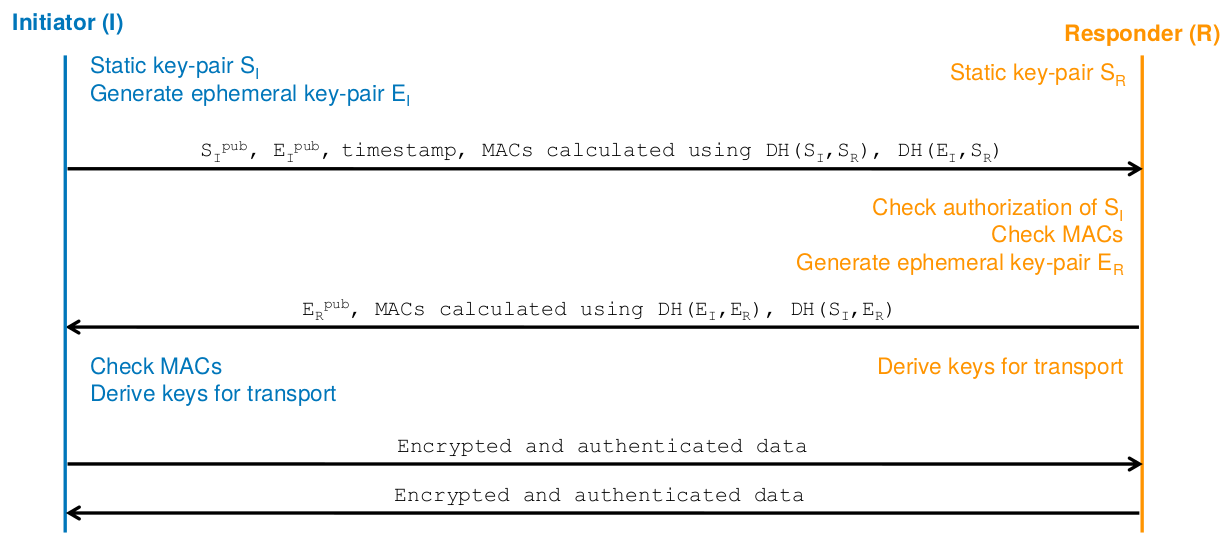
\includegraphics[width=1\linewidth]{figures/wireguard_handshake}
	\caption{WireGuard 1-RTT handshake}
	\label{fig:wireguardhandshake}
\end{figure}

The WireGuard protocol is connectionless. A series of timers, both based on message counts and time, are used to steer key renegotiation, handshakes and session termination. The strict key rotation timers \texttt{(REKEY\_AFTER\_MESSAGES, REKEY\_AFTER\_TIME)} and the ephemeral
ECDH session key exchange guarantee PFS.

\subsubsection{DoS protection}

Since VPN servers need to do expensive crypto, they are susceptible to (D)DoS attacks. A WireGuard implementation can choose to respond with a cookie instead of processing the handshake: the initiator will then use this cookie as a key for computing HMACs of their message. The cookie mechanism of IKEv2 is very similar to the one just described. However, an important difference between the two is that Wireguard requires an additional MAC on the handshake message — using the public key of the responder as HMAC key. This allows the responder to stay completely silent — not responding even with a cookie — unless the initiator knows its public key. (Remember that “public” key do not need to be publicly accessible, often they are not).

\newpage

\section{Anonymous communication systems}

Why are VPNs not enough? VPN server still sees metadata such as srcIP, dstIP, ports, metadata etc. We need something stronger for anonymous communication. 

\subsection{Terminology: “anonymity”}

\vspace{-\topsep}
\begin{itemize}
	\setlength{\itemsep}{0pt}
	\setlength{\parskip}{0pt}
	\item Sender anonymity: adversary knows receiver, may learn message, sender is unknown. The sender anonymity set is the set of all possible senders, which can be used as a (rough) metric. A small set means little anonymity.
	\item Receiver anonymity: Adversary knows sender, may learn message, receiver is unknown. The sender needs a return address: the receiver provides a token (since the sender doesn't know the receiver) and the token will be used to direct the message. Receiver anonymity set is the set of all possible receivers.
	\item (Sender-receiver) unlinkability: Adversary knows senders, knows receivers, link between senders and	receivers is unknown. Multiple users need to communicate at the same time.
	\item Unobservability: Adversary cannot tell whether any communication is taking place.
\end{itemize}
\vspace{-\topsep}

\noindent The following holds: $Unobservability \rightarrow Anonymity \rightarrow Unlinkability$

\subsection{How to send a message anonymously}

\subsubsection{Broadcast}

Receiver anonymity is guaranteed, sender can be de-anonymized (localization through triangulation)!. Alternative: hijacked connection (burner phone, hacked WiFi, network ID ≠ personal sender ID).

\subsubsection{Mixnets}

Simple idea: use a proxy or VPN. The proxy has to be trusted $\rightarrow$ to avoid fully trusting the proxy: Layered encryption. However, the adversary may be able to link inputs
and outputs (timing)!\\\
The proxy should perform \textbf{batching and mixing}. Batching: collect a number of messages
before forwarding (threshold). Mixing: change the order of (mix) the messages.\\
An adversary can still mount an intersection attack: Often, users only communicate with a
small subset of other users. Idea: every time a message is seen by the target, register the sets of destinations. To achieve full unobservability, use \textbf{cover traffic}, both for sending and receiving. Now we are fully anonymous... as long as the mix is trusted!. We should use multiple mixes to avoid single point of failure (cascade). Each mix should only know its direct neighbor and only the first mix should know the sender and only the last mix should know the receiver.\\
\indent How do we handle return addresses? Alice prepares a return address and encloses it in her first message. That address contains layered information.

\subsection{Circuit-based systems (AKA onion-routing system)}

Mix-nets are very secure but very slow. We want a system that can support web browsing. Main ideas: use layered encryption, no batching and mixing, no cover traffic. Flow-based: establish a virtual circuit (keys) once per flow, reuse it for all packets in the flow using only symmetric key crypto. The threat model is constrained: only a local adversary (e.g. ISP) which cannot launch confirmation attacks.\\
\indent \textbf{Terminology:} Circuit-based anonymous communication systems, commonly known as Onion Routing Systems. The nodes are called relays (also nodes or routers). The virtual circuit is also called tunnel.

\subsubsection{Circuit setup}

The sender negotiates shared keys with all relays on the path (this requires expensive asymmetric key cryptography).\\
\noindent \textbf{Direct circuit setup:} a packet is sent through the whole system and returned and at each step the state is generated. The encryption keys of data are only based on public keys of relays. Thus (immediate) FS does not hold since no ephemeral information is used.\\
\noindent \textbf{Telescopic circuit setup:} Keys are negotiated one relay at a time. The circuit is “extended” by one hop at a time (that’s why it is called telescopic). Ephemeral session keys are negotiated before the circuit is extended. This setup is slower... but it offers immediate forward secrecy: As soon as the circuit is closed, the session keys are deleted.

\subsubsection{Data forwarding}

The sender has established a circuit (keys and per-link IDs). A data packet is encrypted as usual (layered encryption). The ID of the next relay is added in clear text. To protect against network adversaries, links can be encrypted (TLS).

\subsubsection{Circuit tear-down}

Can be initiated both by sender and by intermediate relays. The sender communicates the tear-down to one relay at a time, starting from the furthest away. The exit relay may tear down the circuit if a corrupt packet is detected, or some other attack. Circuits have a limited lifetime, so they will eventually be destroyed.

\subsection{Attacks on circuit-based anonymous-communication systems}

Many attacks have been proposed, however for many it is unclear if they fit the standard threat model. Some of them are practical, requiring limited resources. Others are only achievable by state-level adversaries (Five Eyes).

\subsubsection{Fingerprinting}

One general attack is fingerprinting. This can be done in multiple ways:

\vspace{-\topsep}
\begin{itemize}
	\setlength{\itemsep}{0pt}
	\setlength{\parskip}{0pt}
	\item Passive traffic analysis: The adversary observes the edges of the network, recording traffic patterns.
	\item Active traffic analysis: 
	\begin{itemize}
		\item The adversary actively modifies packet timings: Inter-packet timings (delaying/reordering packets), packet drops also possible but detectable
		\item Flow watermarking: inject one bit of information (marked or not)
		\item Flow fingerprinting: inject multiple bits (e.g., sender IP address!)
	\end{itemize}
	\item Website fingerprinting: Many websites have a distinct pattern of traffic they receive and send. Adversary can keep a database of patterns and compare traffic recorded from a single observation point (ISP, WiFi users,...)
\end{itemize}
\vspace{-\topsep}

\noindent There are two possible approaches on how to defend against fingerprinting:

\vspace{-\topsep}
\begin{itemize}
	\setlength{\itemsep}{0pt}
	\setlength{\parskip}{0pt}
	\item Randomization: make the fingerprint look random, each user always has a new, random fingerprint.
	\item Uniformity: make all the fingerprints look the same, all the users share a common	fingerprint. This is what the TOR browser tries to enforce. All Tor Browser user supposedly share the same fingerprint, increasing their anonymity set. Numerous patches are used to limit plugins, ask permission for HTML Canvas, restrict WebSockets, reduce available fonts, standardize the User-Agent header, and limit many other fingerprinting techniques. Even window size is considered sensitive: the browser will warn you if you attempt to maximize its window (you would leak the size of your monitor).
\end{itemize}
\vspace{-\topsep}

\noindent In order to prevent fingerprinting, you should omit \textit{everything} that makes you stand out: don't install any plugins, never use TOR in fullscreen mode (gives away your screen resolution), don't type inside the browser, type inside a text-editor and copy-paste messages into webforms, etc.

\subsubsection{Higher-layer attacks}

\vspace{-\topsep}
\begin{itemize}
	\setlength{\itemsep}{0pt}
	\setlength{\parskip}{0pt}
	\item OS Network stack fingerprinting (OS, browser, window size, user-agent, browser plugins, etc.)
	\item Most deanonymization is still done through other means: Trick user into downloading malware, trick user into downloading file that will access the Internet directly, analyze user behavior like texts.
\end{itemize}
\vspace{-\topsep}

\noindent To achieve anonymity, all layers need to be anonymized: Any gap will break anonymity!

\subsection{TOR}

TOR basics:

\vspace{-\topsep}
\begin{itemize}
	\setlength{\itemsep}{0pt}
	\setlength{\parskip}{0pt}
	\item Circuits established over 3 relays
	\item Telescopic setup (forward secrecy!)
	\item Per-hop TCP, established on the fly to avoid TCP stack fingerprinting
	\item Per-hop TLS (except on the last hop). Multiple circuits over same TLS connection. End-to-end HTTPS is possible.
	\item Main tool: Tor browser (Firefox)
\end{itemize}
\vspace{-\topsep}

\noindent TOR additional features:

\vspace{-\topsep}
\begin{itemize}
	\setlength{\itemsep}{0pt}
	\setlength{\parskip}{0pt}
	\item Exit policies (exit can restrict the destinations	they connect to)
	\item Multiple streams per circuit (helps with performance, weakens anonymity)
	\item Censorship resistance (bridges)
	\item Hidden services: Provide receiver anonymity, use .onion URL (not in DNS). The name is the hash of the HS’s public key.
\end{itemize}
\vspace{-\topsep}

\subsubsection{Cells}

If a relay obtains a cell: it looks up keying material from circuit id and will decrypt the payload which contains sets of fields. The relay then checks the digest and if it matches it looks at the cmd.

\begin{figure}[hb]
	\centering
	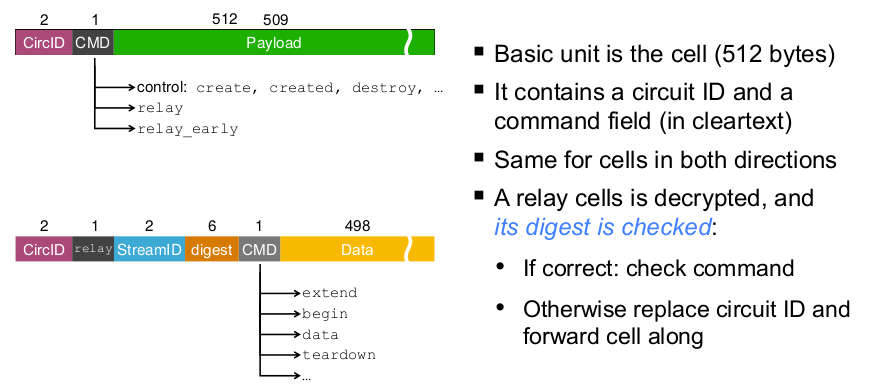
\includegraphics[width=0.7\linewidth]{figures/tor_cell}
	\caption{TOR cell}
	\label{fig:torcell}
\end{figure}

\subsubsection{Directory authorities}

How do the clients know what relays there are? 10 directory authorities (servers) running a consensus algorithm. The authorities track the state of relays, store their public keys. Client software (Tor browser) comes with a list of the authorities’ keys (If an adversary can supply the list, de-anonymization is trivial!). A client accepts a consensus document if signed by ≥ 50\%. The centralized authorities are an important weakness of Tor. An adversary compromising 5 authorities can compromise Tor. Every relay periodically reports a signed statement (state, stats.) DAs also act as bandwidth authorities: verify bandwidth of nodes.\\
Sybil protection: DAs limit the number of relays per IP subnet.

\subsubsection{Censorship resistance in Tor}

The Tor network contains a number of bridge relays (or bridges). Not (all) publicly listed, instead distributed through friends networks. This is used to circumvent censors which black-list Tor relays. Problem: deep packet inspection allows detection of Tor traffic
Solution: obfuscate the traffic (pluggable transports)

\subsubsection{Circuit setup}

Who is authenticated on the first hop? Alice is \textit{not}. The entry guard is since Alice encrypted her ephemeral DH value $g^{x_1}$ with the entry guard's pubKey. The entry guard then sends back $g^{y_1}$ and a hash of $g^{x_1y_1}$ which it can only do if it was able to decrypt $g^{x_1}$ which it can only do if it has the privKey.
\begin{figure}[hb]
	\centering
	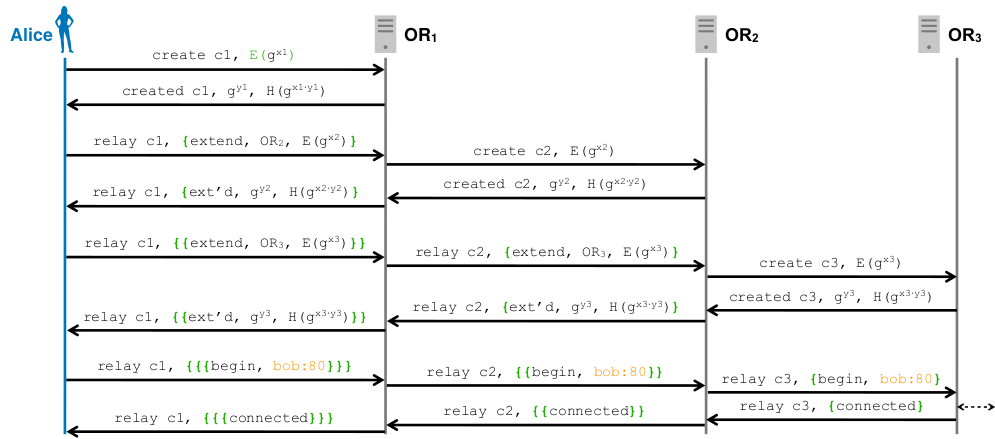
\includegraphics[width=0.9\linewidth]{figures/tor_circuit_setup}
	\caption{Circuit setup with three hops}
	\label{fig:torcircuitsetup}
\end{figure}

\section{DNS Security}

The Internet is a critical infrastructure, yet its operation depends on the fundamentally insecure DNS. DNS provides a mapping of names to resources of several types. However, DNS, as a robust key protocol of the Internet, is also a formidable attack vector for cyber criminals:

\vspace{-\topsep}
\begin{itemize}
	\setlength{\itemsep}{0pt}
	\setlength{\parskip}{0pt}
	\item DNS helps cybercriminals to setup services that are hard to hunt-down or shut-
	down (Botnets, Fast- \& Domain Flux)
	\item DNS helps building hidden channels (tunneling)
	\item is abused for powerful denial of service attacks
	\item is abused for various impersonation attacks
\end{itemize}
\vspace{-\topsep}

\subsection{Domain Name System (DNS)}

DNS uses hierarchical namespaces to scale: tree structure down from root level ".", to top-level domains (TLD, e.g. .com) to second-level domains (SLD, e.g. google.com). A fully qualified domain name (FQDN) for example is mail.ethz.ch. The hierarchy descends from right to left. Domains are namespaces: verything below .com is the \textit{com} domain, everything below .ibm.com. is the \textit{ibm.com} domain.

\begin{figure}[hb]
	\centering
	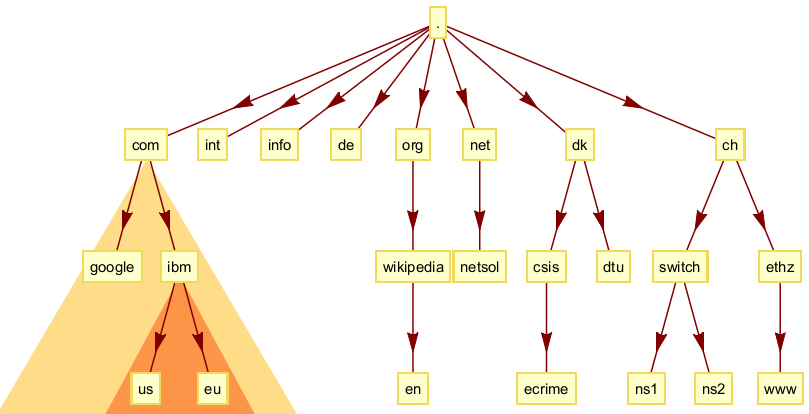
\includegraphics[width=0.6\linewidth]{figures/dns_namespace_hierarchy}
	\caption{DNS Namespace Hierarchy}
	\label{fig:dnsnamespacehierarchy}
\end{figure}

\noindent \textbf{DNS protocols \& elements}

\vspace{-\topsep}
\begin{itemize}
	\setlength{\itemsep}{0pt}
	\setlength{\parskip}{0pt}
	\item Protocol: simple client-server protocol, operating on TCP/UDP port 53. No encryption, authentication nor integrity built into original protocol.
	\item Name server: Servers that map names to objects (= resource records RR). Authoritative: server is authoritative for a specific zone. Caching/Resolver: server resolves domains recursively, caches	results.
	\item Resolver: Client side of DNS resolution, responsible for initiating and sequencing the queries that ultimately lead to a full resolution. Stub resolver: piece of software running on a client that sends recursive DNS requests to a recursive resolver. Recursive resolver: processes DNS resolution iteratively to	provide full answer: it contacts all the different servers at the different domain levels to get the final answer.
\end{itemize}
\vspace{-\topsep}

\noindent Each DNS response has a TTL. Caching resolvers will redo a recursive lookup once the TTL for a cached response has expired. A shorter TTL leads to shorter living cache entries, leading to faster refreshes for end users in case of an update. However, this means that there will be more load on the DNS servers for doing the recursive lookup again.

\subsubsection{Root servers}

DNS root name servers are the key to the Internet kingdom: the DNS root zone is served by 13 root server clusters which are authoritative for queries for the top level domains. Every name resolution in the Internet either starts with a query to a root server, or, uses information that was once obtained from a root server. DNS root name servers have the official names a.root-servers.net to m.root-servers.net. They only resolve the IP addresses for the top-level name servers (TLD).

\subsubsection{Top-Level name servers}

A domain name registrar is an organization that manages the reservation of second-level Internet domain names (SLD) below a given top-level domain (TLD). A domain name registrar must be accredited by a top-level domain registry and/or a country code top-level domain (ccTLD) registry. Based on the domain registration database, the top-level name server points resolvers to the authoritative name server of the SLD.

\subsubsection{Authoritative Domain Server}

The authoritative name server for a second-level domain is managed by private entities or on behalf of private entities that have registered a domain name. The authoritative name server has all records for a zone configured and can provide the final / authoritative information.

\subsubsection{Name Server Roles}

\begin{figure}[hb]
	\centering
	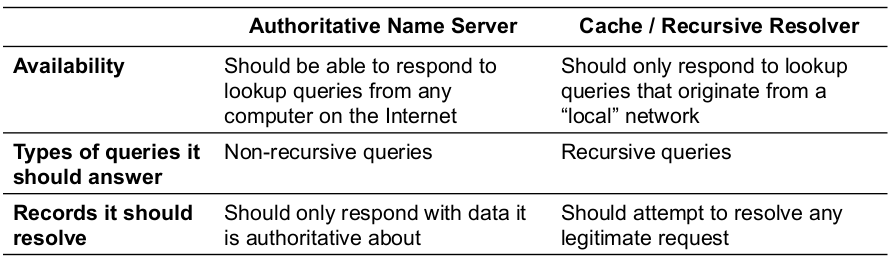
\includegraphics[width=0.7\linewidth]{figures/dns_name_server_roles}
	\caption{DNS - Name Server Roles}
	\label{fig:dnsnameserverroles}
\end{figure}

\subsection{DNS spoofing}

\textbf{Attack Methodology:} Insertion of incorrect resolution information by a host that has no authority to provide that information. DNS requests rely on UDP. Each request is assigned a unique identifier (TXID) to help manage multiple requests. DNS server responds, including the same TXID, client ignores responses with different TXIDs.\\
\textbf{Example:} Client requests www.bank.com. If the attacker is on the same network, she can sniff traffic and look for specific DNS requests. As soon as shes sees the request, she can immediately send back a DNS reply for www.bank.com however with a spoofed IP that points to some location she owns. General rule: first reply wins! When to legitimate reply arrives a bit later, it is ignored. Most likely, the attacker is faster: physically closer, she can drop packets, recursive resolution takes a lot of time, attacker could overload resolver. The TXID can be sniffed or guessed.

\subsection{Distributed Reflection / Amplification DDoS}
\label{dns_ddos}

\textbf{Attack Methodology:} DNS queries are typically transmitted over UDP - they are fire and forget. The source IP can be spoofed and the receiver has no way of determining its veracity before responding. The attacker will spoof the srcIP to the victim's IP - the response will thus be reflected to the victim and overload his servers. DNS also is capable of generating a much larger response than query (e.g. \texttt{dig ANY isc.org @x.x.x.x} query is 64 bytes, the response is 3,223 bytes). There are many powerful and well connected DNS servers, which can be abused to redirect large DNS responses to any target. The key to this attack are \textit{open} DNS resolvers (recursive resolver that replies to any DNS query, coming from any device
on the Internet).\\
\noindent \textbf{Key ingredients of a reflection/amplification attack:} stateless protocol (UDP), can spoof the srcAddr (reflection), small request generates large response (amplification). Other protocols that also fulfill these criteria: memcached, NTP.\\
\noindent \textbf{Mitigation:} Source IP verification (reject packets with source addresses not reachable via the actual packet’s path), disable recursion on authoritative name servers, limit recursion to authorized clients, Response Rate Limiting (RRL).\\
However, the main mitigation is hosting a service on different locations in the internet, s.t. it gets harder for an attacker to target all possible locations. Using BGP anycast, the same IP address is advertised on different locations on the internet.\\
A user is directed to the nearest service location. This helps to distribute the load on different sites. There are CDN services like Akamai or CloudFlare that offer this as a service.

\begin{figure}[hb]
	\centering
	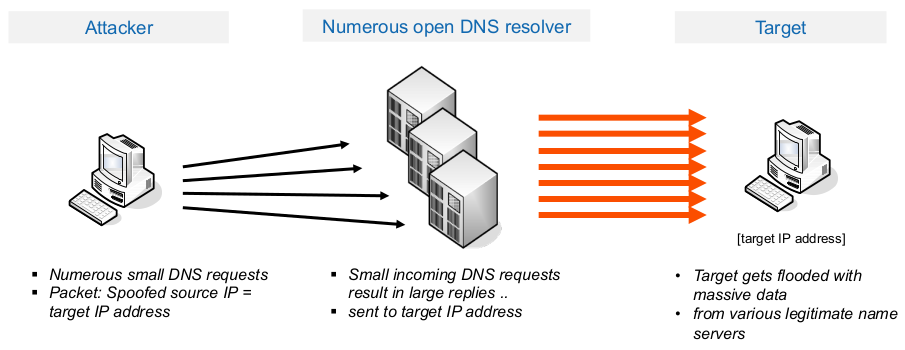
\includegraphics[width=0.7\linewidth]{figures/dns_reflection_amplification_ddos}
	\caption{Distributed Reflection / Amplification DDoS}
	\label{fig:dnsreflectionamplificationddos}
\end{figure}

On TCP, this attack would not work as is since the second message after the TCP SYN is not the DNS response but the TCP SYN ACK. The TCP ACK would go to the victim (due to the srcIP spoofing). The DNS response would be the second message sent by the server. However, the attacker could reply with the third handshake message + payload after inter-epting the replies and dropping them. If the attacker is not Dolev-Yao, which is often the case, the attack would become tricky to perform.

\subsection{DNS Cache Poisoning}

\textbf{Attack Methodology:} Attacker abuses caching capability of domain name system. Inject faked Domain\textgreater IP information into cache of caching name server. Subsequent requests by any user to this server are served this fake information from cache.\\
\textbf{Example:} Attacker owns authoritative name server for bad.com and tricks user to resolve bad.com (phishing, hacked site, attachment, hidden picture, ..). Attacker adds multiple resolution entries for e.g. bank.com into the \texttt{ADDITIONAL SECTION} of the DNS reply  for bad.com. The client will cache this information even though he didn't ask for it.\\
\noindent \textbf{Mitigation:} The example attack is no longer really a problem since software no longer accepts entries from additional section which are for different domains.

\subsection{DNS/Domain Hijacking}

\textbf{Attack Methodology:} Domains are registered with a domain registrar. The DNS information is as secure as the Web App, backend processes, or the passwords of the registrar and the domain owner. An attacker could for example hack the web app of the domain registrar (e.g. godaddy, namecheap, etc.), brute-force user passwords (or get it from data breach) and then manipulate the domain registration entries directly at the registrar (change name servers, and password of registrars Web App).\\
\textit{Your DNS security is as good as the security of the domain registrar, and your credentials.}

\subsection{Local Host / Network LAN \& WAN}

\textbf{Attack Methodology:} Manipulate DNS settings on local host, or provisioning of DNS settings in local network. Have target point to attackers name server.Various attack vectors:

\vspace{-\topsep}
\begin{itemize}
	\setlength{\itemsep}{0pt}
	\setlength{\parskip}{0pt}
	\item Network attack:
	\begin{itemize}
		\item WAN: Attack poorly protected client router of Internet Service Providers (ISP)
		\item LAN: Attack the DHCP exchange in local network. DHCP has no authentication and includes the default name server -\textgreater spoof it. Again, the attacker will be able to outpace the DHCP response of the DHCP server.
	\end{itemize}
	\item Host Attack: Upon compromise of target, manipulate local hosts file (e.g. \texttt{/etc/hosts} for linux) (e.g. after infection). The attacker could for example add a static mapping for www.bank.com to an IP she owns. Malware often adds static mapping to hosts file for antivirus domains (e.g. map to loopback). This way, signatures are not updated.
	\item DNS Changer Botnet: Botnet changes DNS settings on infected hosts. Name server configuration now points to name server of attacker. Possible exploits are ad manipulation (Google ads), phishing (credit cards, online banking) or selling software (fake iTunes shops).
\end{itemize}
\vspace{-\topsep}

\subsection{Botnet Control - Controlling compromised machines}

Cyber criminals organize compromised machines and devices in centrally controlled botnets, consisting of thousands or millions of agents/bots. Bots are used to send spam, DDoS attacks, banking and click-fraud, bitcoin mining, etc. Criminals want to control their botnets and protect their infrastructure from take-down attempts and competitors.\\
\textbf{Botnet management requirements (criminals view):}

\vspace{-\topsep}
\begin{itemize}
	\setlength{\itemsep}{0pt}
	\setlength{\parskip}{0pt}
	\item Bot must receive new instructions and malicious capabilities ..
	\item Robustly manage 10,000+ globally distributed bots ..
	\item Botnet shall be resistant to hijack and shut-down attempts ..
\end{itemize}
\vspace{-\topsep}

\begin{figure}[hb]
	\centering
	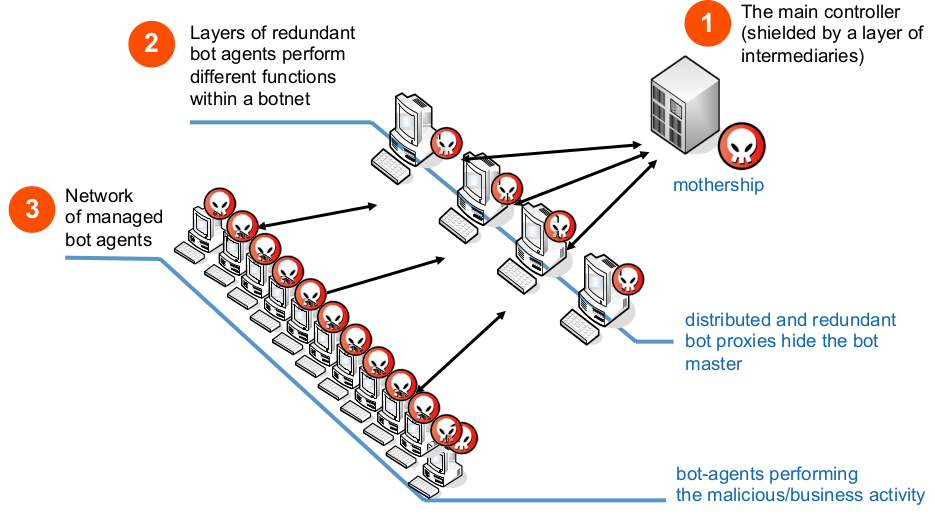
\includegraphics[width=0.7\linewidth]{figures/dns_botnet_architecture}
	\caption{DNS Botnet architecture}
	\label{fig:dnsbotnetarchitecture}
\end{figure}

\noindent The ability of a bot agent to locate the command and control (CnC) infrastructure
is a critical requirement for maintaining control of the entire botnet. However, criminals want to evade law enforcement. By using \textit{fixed IPs} it would be easy to identify bot agent and controller and blocking the botnet would be easy (one firewall rule). By using \textit{fixed domains} it would be easy to identify bot agent, harder to identify controller. Shutting down the botnet would also be harder (DNS caches). More flexibility is obtained through IP flux or domain flux: domain names and/or IP addresses change frequently both technologies are extensively used by professional botnet operators very dynamic, moving target, hard to shut down botnet.

\subsubsection{Fluxing Approaches}

A CnC resource with a given domain name (FQDN) is mapped to a new set of IP addresses as often as every few minutes: a bot agent connecting to the same FQDN actually connects to a different CnC server every 3 minutes this rapid changing aspect is commonly referred to as “Fast-Flux” the IP of unresponsive CnC nodes are taken out of flux and availability is always maintained (Quality of Service).

\vspace{-\topsep}
\begin{itemize}
	\setlength{\itemsep}{0pt}
	\setlength{\parskip}{0pt}
	\item \textbf{IP Flux:} frequent change of IP address information related to a particular fully-qualified domain name (FQDN). Example: cnc.net \textgreater multiple changing IP addresses.
	\item \textbf{Domain Flux:} frequent change and allocation of multiple fully-qualified domain names (FQDN). Example: cnc.net, cnc.ru, abc.com, xyz.ch \textgreater multiple changing IP addresses. Each bot uses a domain generation algorithm (DGA) to periodically compute a list
	of new domain names. From a practical standpoint, domain flux generates a list of “rendez-vous” points that may be used by the bot masters to control their bots.
\end{itemize}
\vspace{-\topsep}

\subsection{DNS over HTTPS (DoH)}

DOH would solve some attacks on DNS such as DNS spoofing, mass-logging of DNS requests, DNS amplification/reflection, cache poisoning, etc. However, there are disadvantages. With DOH, local caches are no longer possible – each query needs to reach the remote DoH resolver. In the case of large providers, load and latency are not a problem: anycast is used to respond to the queries in a geographically distributed way. However, this concentrates even more power in the hands of a few companies (Google, Cloudflare, etc.); the internet gets even more centralized.

\subsection{Domain Name System Security Extensions (DNSSEC)}

DNSSEC attempts to add security, while maintaining backward compatibility to the
existing DNS. DNSSEC is a set of extensions to DNS to provide resolvers: origin authentication of DNS data, authenticated denial of existence, integrity. But not availability or confidentiality.\\
DNSSEC zone data is digitally signed using a private key for that zone. A DNS server receiving DNSSEC signed zone data can verify the origin and integrity of the data by checking the signature using the public key for that zone.\\
\textbf{Process:} (1) Each DNS zone signs its data using a private key (recommended to do offline). (2) A query for a particular record returns: The requested resource record set, a signature (SIG) of the requested resource record set. (3) The resolver authenticates response using public key.

\begin{figure}[hb]
	\centering
	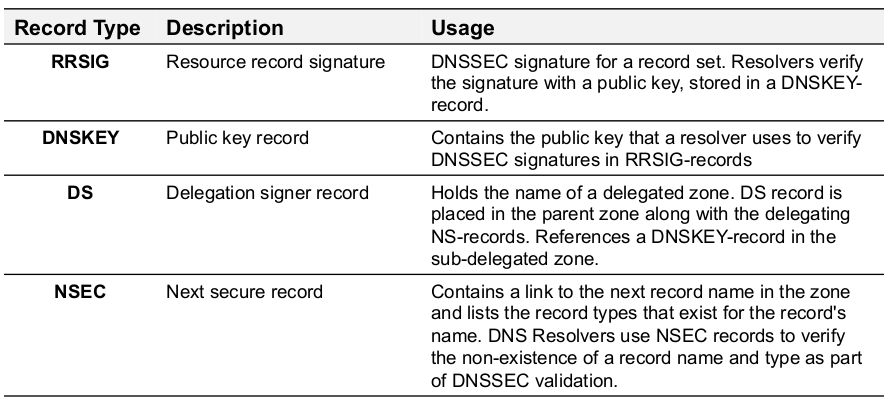
\includegraphics[width=0.8\linewidth]{figures/dnssec_resource_records}
	\caption{DNSSEC Resource Records}
	\label{fig:dnssecresourcerecords}
\end{figure}

\noindent \textbf{DS record:} The DS record contains a hash of the KSK (key signing key) belonging to the
child zone. Once the DNS resolver knows the contents of DS, it can retrieve the KSK and ZSK (zone
signing key) belonging to the child zone. KSK is checked against DS. ZSK is validated using
the KSK. Finally, if the child zone is the actual target of the query, the answer
can be checked by using the ZSK.

\newpage

\section{Firewalls, IDS \& Detection \& Evasion}

\subsection{Firewalls}

A firewall is a system used to protect or separate a trusted network from an untrusted network, while allowing authorized communications to pass from one side to the other.

\vspace{-\topsep}
\begin{itemize}
	\setlength{\itemsep}{0pt}
	\setlength{\parskip}{0pt}
	\item \textbf{Network Firewall:} Network firewalls are a software appliance running on specific hardware or as virtual instance that filter traffic between two or more networks.
	\item \textbf{Host Firewall:} Host-based firewalls provide a layer of software on one host that controls network traffic in and out of	that single machine.
\end{itemize}
\vspace{-\topsep}

\noindent Host based firewalls have context, know exactly what is running on a host. This allows for more fine-grained decisions. Host based firewalls are good for mobile devices (e.g. phones). Network firewalls are good if you e.g. can't install a firewall on a device (e.g. printer).\\

\vspace{-\topsep}
\begin{itemize}
	\setlength{\itemsep}{0pt}
	\setlength{\parskip}{0pt}
	\item \textbf{Stateless Firewall:} look at each packet on the network layer individually, no state maintained. Decisions based on packet header information. This is fast, scalable and simple but very limited.
	\item \textbf{Stateful Firewall:} keep also track of the state of the network connections, decision also based on session state. This is more powerful but: state explosion, inconsistencies, state for UDP.. The problem with state explosion: an attacker can exhaust the memory of a firewall. Then, the default rule matches: if default accept: all traffic is allowed. If default deny: server is DoSed.
\end{itemize}
\vspace{-\topsep}

Firewalls have ingress (incoming traffic) and egress (outgoing traffic) rules. Packets can be dropped (silent) or rejected (ICMP reply). Firewall rules are processed in order: the first rule that matches is picked. Thus, ordering of rules is very important.\\

\textbf{Problems:} Firewalls \textit{need} to allow traffic (HTTP(S), SSH, various new protocols that use various ports, e.g. instant messaging). Thus, some malicious traffic will go through. We need an advanced notion of Firewalls.

\subsubsection{Next Generation Firewall (NGFW)}

\textbf{Functionality:} deep packet (content) inspection, take application and protocol state into
account for security decision. This allows for protocol \& application awareness but requires support for many (badly documented) protocols, has performance and scalability issues and introduces inconsistencies between host/app and FW.

\subsubsection{Web Application Firewall (WAF)}

Protect web-based applications from malicious requests. Request filtering: request pattern, SQL injection, XSS, buffer overflow attempts, etc. Often implemented as a reverse proxy.

\subsubsection{Organizational Challenges}

Managing and maintaining firewall rules in a company is challenging. Firewall rules are complex and if the employee that created them leaves, someone else has to understand the monster. Further, security and network operation teams have opposing interests: security team wants to provide secure access, network team wants to provide high availability.

\subsection{Intrusion Detection \& Prevention}

\textit{Make decision whether some traffic is good or bad.}

\noindent This faces many challenges: encrypted traffic (can't inspect content, only headers and statistical analysis), high number of false positives, high link speeds, induced latency, application level attacks (JavaScript, ..), etc.

\noindent Accurate = right direction, on target. Precise = clustered values with low scatter.\\

\textit{“It is better to be roughly right than precisely wrong.”}\\

\noindent Never believe an IDS that advertise perfect detection with 0\% FNR or 0\% FPR:

\vspace{-\topsep}
\begin{itemize}
	\setlength{\itemsep}{0pt}
	\setlength{\parskip}{0pt}
	\item \textbf{0\% FNR:} Always predict 'Attack!'
	\item \textbf{0\% FPR:} Always predict 'No attack!
\end{itemize}
\vspace{-\topsep}

\noindent The difficulty: Build a detector with optimal balance between FP and FN. FNR and FPR should never be considered in isolation. Ideally, consider a joint detection metric such as the F1 score.\\
Accurate detection is very challenging when rate of attacks is very low. If we have lots of traffic but very few attacks, we'll have lots of false positives, which lowers trust in the detector. 

\subsection{Detection Methods}

\vspace{-\topsep}
\begin{itemize}
	\setlength{\itemsep}{0pt}
	\setlength{\parskip}{0pt}
	\item Reactive: system can only detect already known attacks
	\item Proactive: system can detect known and yet unknown attacks
	\item Deterministic: system always performs the same given the same input (blacklist, signatures)
	\item Non Deterministic: system detection is fuzzy (heuristics, machine	learning, sandboxing) and depends on current state of the world. The reason for alert is typically not known.
\end{itemize}
\vspace{-\topsep}

\vspace{-\topsep}
\begin{itemize}
	\setlength{\itemsep}{0pt}
	\setlength{\parskip}{0pt}
	\item Signature based systems: Promptly identify and label threat. But I can only identify threats that I've already seen before. Frequent updates to signature database or online lookups.
	\begin{itemize}
		\item One-Dimensional: blacklist/ whitelist (e.g based on MD5 hashes). This is fast and low FPR. But it's reactive and needs frequent updates.
		\item Two-Dimensional: classic regular-expression functions and string matching. This is more flexible and has low FPR and low/medium resource requirements. But it's still reactive and needs frequent updates.
		\item Multi-Dimensional: instead of triggering on a single signature, a	multi-dimensional signature was created. More efficient and effective than single approach.
	\end{itemize}
	\item Sandboxing: Run (potential) malware in a VM and examine its behavior. This is proactive and doesn't need signature updates but is resource intensive and difficult to scale. Malware can further evade sandboxing (e.g. malware could wait for 3 days before becoming malicious).
	\item Machine Learning: Apply supervised and unsupervised machine learning algorithms to detect malicous traffic, malware, etc. Problem with SL models: training data \textit{needs} to be clean (no unknown attacks), otherwise the SL model learns something wrong. With USL models, interpretability is an issue (also with SL).
\end{itemize}
\vspace{-\topsep}

\subsection{Attack methods}

Lots of techniques exist to evade detection:

\vspace{-\topsep}
\begin{itemize}
	\setlength{\itemsep}{0pt}
	\setlength{\parskip}{0pt}
	\item IP Source Spoofing
	\item Artificial Fragmentation: Fragment packets to bypass rules. The FW needs to reassemble packets to obtain a complete picture.
	\item Vulnerabilities: exploit bugs in FW software, firmware, OS
	\item (D)DoS: state explosion, exploit FW default rule
	\item Tunneling/ Covert Channels: data in ICMP pings, DNS request, use VPN
	\item Encodings: Confuse the inspection engine by using encodings that will be ignored by the final application but the engine will see it (e.g. use characters that are not part of base64 -\textgreater will be seen by engine but ignored by base64 decoder)
\end{itemize}
\vspace{-\topsep}

\subsection{Malware Development	\& Detection Evasion}

Basic detection approaches:

\vspace{-\topsep}
\begin{itemize}
	\setlength{\itemsep}{0pt}
	\setlength{\parskip}{0pt}
	\item Static (Signatures): reliable, low FPR, but reactive and reliant on updates
	\item Behavior (Dynamic): proactive, detects unknown threats, but complex and computationally expensive, higher FPR
\end{itemize}
\vspace{-\topsep}

\noindent Malware development lifecycle with detection evasion by design:

\vspace{-\topsep}
\begin{enumerate}
	\setlength{\itemsep}{0pt}
	\setlength{\parskip}{0pt}
	\item Develop new malware with desired functionality
	\item Automatically create an array of unique/permutated samples of the	initial malware at massive scale:
	\begin{itemize}
		\item Create serial variants (many different variants of a malware)
		\item trickle release different variants to constantly stay ahead of AV updates
	\end{itemize}

	\item Protect samples from analysis:
	\begin{itemize}
		\item Use \textit{crypter} to encrypt malware s.t. detection systems and static analysis processes are ineffectual.
		\item Upon execution only decrypt sections of code that are in the process of being executed on the victim’s computer.
		\item Use \textit{packers} to make binary files smaller (faster infection), make it more difficult for AV to detect malicious payload. Advanced packers employ polymorphic output capabilities (restructure malware binary everytime it's executed)
	\end{itemize}

	\item Make samples aware of sandboxing/detection technologies
	\begin{itemize}
		\item Use \textit{protector} to add anti-debugging features to malware that prevent security researchers and automated sandbox analysis technologies from dissecting samples.
		\item “protector” technology was originally designed as a DRM protection technology
		\item Protectors detect the use of debuggers or virtualization techniques if seen, the malware then causes different operations
	\end{itemize}
	\item Quality Assurance: Test samples against all current anti-malware solutions before deployment (\texttt{goto 2}):
	\begin{itemize}
		\item Check if the malware is detected by common AV software. Only testing services that do not submit malware samples to antivirus vendor are used (otherwise the malware would already be known).
	\end{itemize}
\end{enumerate}
\vspace{-\topsep}

\noindent The malware used in a targeted attack will not be detected by anti-malware tools at the time of attack – because it was tested beforehand.

\noindent \textbf{Polymorphism technique:} Swapping equivalent code constructs, changing the order of code, insert noise, compiler modulation.

\noindent \textbf{Binders:} Binders are used by malware authors to “embed” and Trojan other software packages (e.g. add trojan to Adobe Photoshop torrent). This helps to propagate malware, trick users into downloading and executing seemingly legit software. 

\subsection{Layered defense}

\vspace{-\topsep}
\begin{itemize}
	\setlength{\itemsep}{0pt}
	\setlength{\parskip}{0pt}
	\item Direct attack: “server-side” exploits, the threat/exploit is executed remotely by the attacker against a vulnerable application and/or operating system
	\item Indirect attack: the threat/exploit is initiated by the vulnerable target. The attacker has little or no controll over when the target user executes the threat.
\end{itemize}
\vspace{-\topsep}

\subsection{Botnets}

Basic components:

\vspace{-\topsep}
\begin{itemize}
	\setlength{\itemsep}{0pt}
	\setlength{\parskip}{0pt}
	\item Bots: devices under control of the attackers – often vulnerable hosts that have been
	infected with a malware.
	\item Command and Control infrastructure: often owned by the attackers, is it used to push
	commands to the bots.
\end{itemize}
\vspace{-\topsep}

\subsubsection{Mirai botnet}
\label{mirai_botnet}

Mirai mainly targeted IoT devices. IoT devices are a very interesting attack vector since there are lots of IoT devices (ca. 10 billion for 2019), they are configure-and-forget (owners don't update them and don't realize when they're compromised) and security is often lacking in IoT devices.\\
Mirai has been used mainly for Distributed Denial of Service attacks. DDoS is much harder to track and take down than a regular DoS. This allows the attacker to hide his identity behind the botnet. Additionally, a DDoS enables the attacker to have a virtually unlimited bandwidth for flood attacks.\\
Mirai infection technique:

\vspace{-\topsep}
\begin{enumerate}
	\setlength{\itemsep}{0pt}
	\setlength{\parskip}{0pt}
	\item Scan: infected device scans network for open Telnet ports (send TCP SYN packets to random IPv4 addresses)
	\item Brute force: the bot tries to log in using 10 random user/pass combinations taken from
	a hardcoded list of 62. These represent default credentials of existing devices.
	\item Report: upon login success, the bot reports the target to a Report Server. It lists IP
	address, type of device (if available) and successful credentials.
	\item Infection: a Loader program gets a detail of the target from the Report Server, connects
	to Telnet and uploads the correct malware binary to the machine.
\end{enumerate}
\vspace{-\topsep}

\noindent Mirai is non-persistent: the binary is loaded into memory and immediately deleted from disk. Rebooting will remove the malware, but the device can still be reinfected. This makes detection and forensic analysis more difficult, especially for IoT devices.\\
Mirai infected devices were fingerprinted by the fact that Mirai generated probe packets had their sequence number equal to the IP of the scanned device. Probability of this happening is $\frac{1}{2^{32}}$.

\subsection{Stuxnet}

Stuxnet is the first (publicly know) cyberweapon - a complex malware, widely believed to have targeted uranium enrichment infrastructure in Iran. Stuxnet used various infection vectors such as WinCC machines, network shares, print spooler zero-day, removable drives (to jump airgaps). Stuxnet installed a driver, signed with a legitimate Realtek certificate. This driver intercepts I/O requests, making the files installed by the malware invisible. It also registers as a boot start service, acting as load point at reboots. This driver behaves very much like a legitimate Windows driver: this, and its legitimate Realtek signature, make it very hard to detect even for an experienced sysadmin. Stuxnet would survive manual inspection, OS updates and antivirus scans. This required legitimate certificates. Using fake certificates would have also been possible but surviving system updates would become harder. Hiding in plain sight is often a winning strategy. Stuxnet often injected itself into the privileged antivirus process to ease the infection. Depending on the antivirus, it alternatively ignored it and injected itself in a Windows system process. 

\section{Internet of Things (IOT)}

\label{iot}

Safety = protection against accidents (environment doesn't adapt to bypass safety measures). Security = protection against targeted attacks (adaptive attacker).\\

The biggest challenge in cyber security is the misconception of risk. Humans perceive fire as risky. (Most) humans don't perceive their smart toaster as a risk, although it is. People need highly visible incidents before they act.\\
We no longer live in a complicated system but in a complex adaptive system \textbf{CAS}:

\vspace{-\topsep}
\begin{itemize}
	\setlength{\itemsep}{0pt}
	\setlength{\parskip}{0pt}
	\item Connectivity: A decision in one part of the system will affect other related or distant parts.
	\item Sensitive dependence: Non-linearity, cascades.
	\item Emergent order: Emergent and unpredictable behavior, which cannot be predicted even with full knowledge of all elements.
\end{itemize}
\vspace{-\topsep}

\noindent We have to adopt to permanent change, high dynamics, and decreased predictability.\\

Humans and nature take different approaches to handle unpredictability: humans prevent shock (reliant on accuracy, fragile, short-term strategy), nature absorbs shocks (anti-fragile, long-term strategy). Degree of optimization: Tradeoff between short term gains vs. long term survival.

\noindent Consequences from properties of CAS for cyber security: new \& innovative attacks, predicability of attacks decreases, remote effects \& cascades.

\subsection{IoT (and IIOT, ICS, SCADA, OT\&OT)}

\vspace{-\topsep}
\begin{itemize}
	\setlength{\itemsep}{0pt}
	\setlength{\parskip}{0pt}
	\item Information Technology (IT): The entire spectrum of technologies for information processing, including software, hardware, communications technologies and related services. Generally does not include embedded devices.
	\item Operational Technology (OT): Hardware and software that detects or causes a change through the direct monitoring and/or control of physical devices, processes and events in the
	enterprise.
	\item Industrial Control Systems (ICS): Systems that are used to monitor and control industrial processes focused on automation, computerized monitoring and control of physical industrial processes (e.g. oil refining). Typically considered to be mission-critical applications with a high-availability requirement.
	\item Internet of Things (IOT): High level concept of a global network of “smart” physical objects of various kinds (wearables, smart toaster,...)\
	\item Industrial Internet of Things (IIOT): Subset of IoT specific to industry (e.g. advanced field sensors)
	\item Critical Infrastructure (CI): Critical infrastructure refers to processes, facilities, technologies, networks and systems (including IIOT and ICS) that control and manage essential services. Disruptions of critical infrastructure could result in catastrophic consequences.
\end{itemize}
\vspace{-\topsep}

\noindent Our world is quickly changing in an irreversible move towards IT/OT convergence. Extending security models to include the OT domain introduces many challenges: conventional IT security thinking hasn't reached (I)OT industry yet, OT devices must not be assumed to be ‘just another end point’.

\noindent \textbf{Key Differences between IT and OT:}

\begin{tabular}{|c|c|}
	\hline 
	OT& IT \\ 
	\hline 
	\textbf{availability \& integrity} & \textbf{confidentiality} (integrity, availability)  \\ 
	at edge of the network & at the center of the network (consumer at edge) \\
	long life cycle & short life cycle \\
	slow response to threats & rapid response to threats \\
	Limited data capacity and computing power & High data capacity and computing power \\
	Safety Operations is critical & Few safety critical operations \\
	\hline 
\end{tabular} 

\subsection{IOT	Attack Surface}

IOT connects innumerable everyday devices and systems. Previously closed systems are opened up to remote access and control. This opens up a large attack surface:

\vspace{-\topsep}
\begin{itemize}
	\setlength{\itemsep}{0pt}
	\setlength{\parskip}{0pt}
	\item Device: insecure software, lacking update mechanism
	\item Communication: insecure communication, weak or no cryptography, lack of authentication
	\item Backend services: Central control, erosion of privacy, data breaches
\end{itemize}
\vspace{-\topsep}

\noindent Further, user perception of risks in cyber security is usually wrong: most users perceive their PC as exposed to malware and fear getting malware but think their smart TV, smart toaster, smart everything (\href{https://twitter.com/internetofshit}{@internetofshit}) are great and don't pose any risks. In reality, the opposite is the case: PC security is rather sophisticated (hardened over 20 years) and we have frequent security updates (e.g.finding a vulnerability in Win10 is hard). But IoT devices ran in isolation for years and only recently became connected. They are designed for high availability and safety, \textit{not} security. Further, IoT devices rarely get security updates. However, the threat environment only gets worse over time, thus we rapidly create a huge future liability with devices lacking an automated and robust protection functionality.\\
To make matters worse:

\vspace{-\topsep}
\begin{itemize}
	\setlength{\itemsep}{0pt}
	\setlength{\parskip}{0pt}
	\item IoT devices typically have a much longer lifetime (1-20+ years) than phones/PCs. That's a long time: vendor could go bankrupt. Solutions: Code escrow (copy source code at trusted third party), open source software
	\item Certification vs. Security: operation critical devices (e.g. flight management system) need certification. However, digital products constantly require security updates which invalidates the certificate. Thus, we need to re-certificate after every patch. BUT: Certification timeline is outpaced by cyber security.
	\subitem \textit{You're doomed if you patch - you're doomed if you don't.}
\end{itemize}
\vspace{-\topsep}

\subsection{Possible approaches to make things better}

IOT security is part of a complex and evolving ecosystem of diverse domains. Technology based security solutions have to complement other domains to achieve the desired security level.

\vspace{-\topsep}
\begin{itemize}
	\setlength{\itemsep}{0pt}
	\setlength{\parskip}{0pt}
	\item \textbf{enforce some minimal security standards and testing for IoT devices}
	\item Design systems with redundancy and resiliency.
	\item Active management of vulnerabilities (coordinated disclosure, bug bounty)
	\item Robust and scalable process to deploy security updates timely and efficiently - on any connected device
	\item Industry-wide systematic security and integrity testing of all critical components
\end{itemize}
\vspace{-\topsep}

\newpage

\subsection{TRENDnet Security Breach}

IP cameras by Trendnet had vulnerability that allowed attackers to view live video stream of any camera. The root directory of the camera’s server had, next to the management directory, another script called mjpg.cgi This script, accessible at \texttt{https://IP\_ADDR/anony/mjpg.cgi}, streamed the captured video in real-time without the need of any authentication. Shodan (\href{https://www.shodan.io/}{shodan.io}) was used by attackers to find IPs with that camera behind.





\label{lastpage} % this must stay here
\clearpage
\addcontentsline{toc}{section}{References}
\bibliographystyle{acm}
\bibliography{refs}

\clearpage
\appendix
\pagenumbering{Roman}

\end{document}
